\chapter{Solver Development}


\section{SPAeCE Algorithm}
\label{sec:spaeceAlg}
In this study, we propose the \textbf{S}ymmetry \textbf{P}reserving, \textbf{A}dvection \textbf{e}xplicit, \textbf{C}onservation of \textbf{E}nergy (\textbf{SPAeCE}) algorithm for transient incompressible flow. The \spaece algorithm is a semi-implicit, projection-like segregated flow solver. To describe the algorithm, let's develop linear system of equations for the mass and momentum conservation following the governing equations Eqs. \eqref{eqn:massCons} and \eqref{eqn:momentumCons} respectively
\begin{subequations}
\begin{equation}
\mathcal{M}\avb{u}_f^{n+1} = \mathbf{0},
\label{eqn:linSysMass}
\end{equation}
\begin{equation}
\mathcal{A}\avb{u}_c^{n+1} = \left( \mathcal{A}^T + \mathcal{A}^S \right)\avb{u}_c^{n+1} = \mathcal{H}(\avb{u}_c^{n+1}) -\mathcal{G}\avb{p}_c^{n+1} + \mathcal{S}^{n+1},
\label{eqn:linSysMom}
\end{equation}
\end{subequations}
where $\mathcal{A}^T$ and $\mathcal{A}^S $ denotes the diagonal coefficient from the discrete temporal operator and spatial operators respectively. $\mathcal{H}$ represents the off-diagonal coefficient matrix, $\mathcal{G}$ denotes the collocated pressure gradient operator matrix and $ \mathcal{S}$ is the summation of all explicit source terms.
 
Unlike a coupled algorithm, in segregated algorithms, separate system of equations for pressure and each velocity components are solved sequentially (i.e. (3+1) system of equations for 3D flow). In such loosely coupled algorithms, time-steps are usually small to keep the segregation error much smaller than the discretization error. The segregated \spaece algorithm has two distinct steps: momentum prediction, and pressure correction. These two steps along with additional steps for the secondary variable(s) transport and overall induced errors are discussed below: 

\begin{enumerate}

\item \textit{Momentum prediction} 

\begin{itemize}

\item \textit{Semi-implicit discretization of momentum equation}
 To advance the flow solution from time $t$ to ($ t+ \Delta t $) i.e. $\avb{u}_c^{n} $ to $\avb{u}_c^{n+1} $, the momentum conservation Eq. \eqref{eqn:momentumCons} is discretized implicitly using the Crank-Nicolson temporal scheme to obtain an approximate velocity field $\avb{u}^{n+1,*}$ as
\begin{align}
\begin{split}
&\frac{\avb{u}_c^{n+1,*} - \avb{u}_c^{n} }{\Delta t}
+ \mathbf{A}( \mathbf{\avb{u}_f^*}) {\avb{u}_c^*} 
+ \mathbf{V} \mathbf{G}_c \avb{p}_c^*
\\
&=\half \left[ 
 \mathbf{M} \nueffb \mathbf{G}_f {\avb{u}_c^{n+1,*}} 
 + \mathbf{M} \nueffb \mathbf{G}_f {\avb{u}_c^*}
\right]
+ \mathbf{M} \left[ \nueffb \left( \mathbf{G}_f^T - 2\mathbf{M}\,\mathbf{I} \right) {\avb{u}_c^*} \right],
\end{split}
\end{align}
 where $\avb{u}_c^{*}$ is an explicit estimation for $\avb{u}^{n+1}$ and $\avb{u}^{n+1, *}$ is the linear system solution which only satisfies momentum conservationFollowing the Crank-Nicolson scheme, the Laplace-like component of the diffusion operator is treated semi-implicitly and rest of the components are treated explicitly. The semi-implicit treatment relives the dissipation CFL number constraint in a low Reynolds number flow or near-wall region where flow is diffusion dominated (see Kim et al. \cite{kim1985}). The linear system for momentum prediction becomes
\begin{align}
\begin{split}
\mathcal{A}\avb{u}_c^{n+1,*} &= \left( \mathcal{A}^T + \mathcal{A}^S \right)\avb{u}_c^{n+1,*} = \mathcal{H}(\avb{u}_c^{n+1,*}) -\mathcal{G}\avb{p}_c^* + \mathcal{S}^{*},
\\
\mathcal{A}^T &= \frac{\mathbf{V}}{\Delta t},
\\
\mathcal{A}^S &= \sumFV \mathcal{H}\mathbf{1_c},
\\
\mathcal{G} &= \mathbf{V} \mathbf{G}_c,
\\
\mathcal{S}^{*} &= \frac{1}{\Delta t} f(\avb{u}_c^{n}, \avb{u}_c^{n-1})  -\mathbf{A}(\avb{u}_f^*) {\avb{u}_c^*} + \mathbf{M} \left[ \nu_{eff} \left( \mathbf{G}_f^T - 2\mathbf{M}\,\mathbf{I} \right) {\avb{u}_c^*} \right],
\label{eqn:linSysMomApprox}
\end{split}
\end{align}
which is symmetric and can be solved with a symmetric matrix algorithm e.g. conjugate gradient method. The $\mathcal{A}^S = \sumFV \mathcal{H}\mathbf{1_c} $ relation originates from the zero-sum rule \cite[Sec. 8.2]{moukalled2015} of the Laplace-like symmetric component of the dissipation operator $\mathbf{D}$, and $\mathbf{1_c} \in \mathbb{R}^n$ is a collocated unit vector.
 
\item \textit{Explicit estimation of primary variables:} The explicit terms approximation method is essential to reduce the approximation error $(\avb{u}_c^{n+1} - \avb{u}_c^{n+1,*})$, particularly in a non-iterative algorithm. For any variable $\phi$, the iterative \piso algorithm \cite{issa1986piso} uses a first order approximation ($\phi^{n+1} \approx \phi^* = \phi^{n}$) in the first iteration. Tukovic et al. \cite{tukovic2018} proposed a linear extrapolation ($\phi^{n+1} \approx \phi^* = (2 \phi^{n} - \phi^{n-1})$) and observed that this approach may cause instability in high Reynolds number flows. Vuorinen et al.\cite{vuorinen2014} also used same technique for a non-iterative Runge-Kutta temporal integration approach. Following the extrapolation approach of Kim et al. \cite{kim1985} and Trias et al. \cite{trias2014}, we followed the Adam-Bashforth like extrapolation approach 
\begin{align}
\phi^{n+1} \approx \phi^* = \phi^{n+ \half} = \half \left( 3 \phi^{n} - \phi^{n-1} \right).
\label{eqn:extrapolation}
\end{align}


\item \textit{Source terms:} Momentum source (or sink terms) such as body forces (e.g. gravitation acceleration, driving pressure gradient, etc.) if present, shall be updated using the approximate pressure $\avb{p}_c^*$ and velocity ($\avb{u}_c^*, \quad \avb{u}_f^*$) fields.


\item \textit{Explicit advection:} Sanderse et al. \cite{sanderse2013} reported that Crank-Nicolson scheme (equivalent to the 2nd order Lobato IIIA scheme) is not exactly kinetic energy conserving. An explicit advection using the extrapolated velocity $ \avb{u}^* = \half \left( 3 \avb{u}^{n} - \avb{u}^{n-1} \right) $ ensures kinetic energy conservation in absence of viscosity. Similar method was also proposed by Spalding \cite{spalding1980} in the SIMPLEST algorithm, Verstappen et al. \cite{verstappen2008} and Trial et al. \cite{trias2014}.

\end{itemize}

\item \textit{Pressure correction}

\begin{itemize}

\item \textit{Update face-normal velocity:}
The approximate face-normal velocity at time $t+1$ can be obtained via the cell-to-face interpolation operator
\begin{align}
\avb{u}_f^{n+1, *} = \shiftCS \avb{u}_c^{n+1, *} \cdot \faceUnitNormal ,
\label{eqn:updateUf}
\end{align}
where $\faceUnitNormal \in \mathbb{R}^m$ denotes the face-normal unit vector for all faces.

\item \textit{Poisson pressure correction:} Subtracting the approximate momentum conserving Eq. \eqref{eqn:linSysMomApprox} from the exact conservation Eq. \eqref{eqn:linSysMom}, we get
\begin{align}
\begin{split}
\avb{u}_c^\prime &= \avb{u}_c^{n+1} - \avb{u}_c^{n+1, *}
\\
\left( \mathcal{A}^T + \mathcal{A}^S \right) \avb{u}_c^\prime &= \mathcal{H}\avb{u}_c^\prime -\mathcal{G}\avb{p}_c^\prime + \mathcal{S}^{\prime},
\\
\mathcal{S}^{\prime} &\approx -\mathbf{A}(\avb{u}_f^\prime) {\avb{u}_c^\prime} + \mathbf{M} \left[ \nueffb \left( \mathbf{G}_f^T - 2\mathbf{M}\,\mathbf{I} \right) {\avb{u}_c^\prime} \right],
\end{split}
\label{eqn:linSysDiff}
\end{align}
where $\avb{u}_c^\prime$ and $\avb{p}_c^\prime$ denotes the velocity and pressure correction respectively. Note that the advection correction is approximated as $\mathbf{A}(\avb{u}_f^{n+1}) {\avb{u}_c^{n+1}} - \mathbf{A}(\avb{u}_f^*) {\avb{u}_c^*} \approx \mathbf{A}(\avb{u}_f^\prime) {\avb{u}_c^\prime}$. The explicit source difference $\mathcal{S}^{\prime}$ becomes very small with good approximation of extrapolated velocity; $\mathbf{A}(\avb{u}_f^\prime) {\avb{u}_c^\prime}$ is small because of its' quadratic nature, and the explicit component of the dissipation is usually minuscule. If explicit source correction $\mathcal{S}^{\prime}$ is ignored, the momentum conservation correction equation becomes
\begin{align}
\left( \mathcal{A}^T + \mathcal{A}^S \right) \avb{u}_c^\prime &\approx \mathcal{H}\avb{u}_c^\prime -\mathcal{G}\avb{p}_c^\prime.
\label{eqn:linSysMomCorrAll}
\end{align}

Following the SIMPLE-Consistent algorithm \cite{vanDoormaal1984}, the velocity correction at any face is approximated as a coefficient-weighted average of the neighboring cell values, i.e.
\begin{align}
\begin{split}
\avb{u}_c^\prime &\approx \frac{\mathcal{H}\avb{u}_c^\prime}{\mathcal{H}\mathbf{1_c}}
\\
\mathcal{H}(\avb{u}_c^\prime) &\approx \avb{u}_c^\prime \, \mathcal{H}\mathbf{1_c}.
\end{split}
\label{eqn:H1}
\end{align}

Substituting the $\mathcal{H}(\avb{u}_c^\prime)$ approximation (Eq. \eqref{eqn:H1} and diagonal coefficient of discrete spatial operator $\mathcal{A}^S = \sumFV \mathcal{H} \mathbf{1_c}$ (Eq. \eqref{eqn:linSysMomApprox}) into the momentum conservation correction Eq. \eqref{eqn:linSysMomCorrAll}, we get
\begin{align}
\begin{split}
\left( \mathcal{A}^T + \mathcal{A}^S \right) \avb{u}_c^\prime &\approx \avb{u}_c^\prime \, \mathcal{H}\mathbf{1_c} -\mathcal{G}\avb{p}_c^\prime,
\\
\left( \mathcal{A}^T + \mathcal{A}^S \right) \avb{u}_c^\prime &\approx \avb{u}_c^\prime \, \mathcal{A}^S -\mathcal{G}\avb{p}_c^\prime,
\\
\mathcal{A}^T \avb{u}_c^\prime &\approx -\mathcal{G}\avb{p}_c^\prime.
\end{split}
\label{eqn:linSysMomCorrCell}
\end{align}

Similarly, equivalent interpolated coefficient matrices for face-normal velocity can be derived and the linear system becomes
\begin{align}
\begin{split}
\mathcal{A_F}^T \avb{u}_f^\prime &\approx -\mathcal{G_F}\avb{p}_c^\prime,
\\
\avb{u}_f^\prime &\approx - {(\mathcal{A_F}^T )}^{-1} \, \mathcal{G_F}\avb{p}_c^\prime,
\\
\mathcal{A_F}^T &= \frac{\mathbf{V}_f}{\Delta t},
\\
\mathcal{G_F} &= \mathbf{V}_f \mathbf{G_f},
\end{split}
\label{eqn:linSysMomCorrFace}
\end{align}

where $\mathcal{A_F}^T$ denotes face-interpolated temporal discretization coefficient matrix and $\mathcal{G_F}$ face-normal gradient coefficient matrix. Substituting the velocity correction from Eq. \eqref{eqn:linSysMomApprox} and taking divergence of the system
\begin{align}
\begin{split}
\mathcal{M} \left[ \avb{u}_c^{n+1} - \avb{u}_c^{n+1,*} \right] &\approx 
- \mathcal{M} \left[ {(\mathcal{A_F}^T )}^{-1} \, \mathcal{G_F}\avb{p}_c^\prime \right].
\end{split}
\label{eqn:linSysMomCorrDiv}
\end{align}

Following the mass conservation linear system Eq. \eqref{eqn:linSysMass}, a poisson equation for pressure correction cab expressed as
\begin{align}
\begin{split}
\mathcal{L} {(\mathcal{A_F}^T)}^{-1} \, \avb{p}_c^\prime &\approx \mathcal{M} \avb{u}_f^{n+1,*},
%\\
%\mathcal{L} &= \mathcal{M} \mathcal{G_F},
\end{split}
\label{eqn:poissonPressure}
\end{align}
where $\mathcal{L} = \mathcal{M} \mathcal{G_F}$ is the coefficient matrix of the discrete Laplace operator defined in the Eq. \eqref{eqn:LaplaceOp}. This equation formulation is similar to the Helmholtz-Hodge vector decomposition theorem used in projection methods pioneered by Chorin \cite{chorin1968}. Although, the linear system for mass conservation (Eq. \eqref{eqn:linSysMass}) is not solved directly, it is indirectly enforced thorough application of the divergence free constraint in the pressure correction Eq. \eqref{eqn:poissonPressure}.

\item \textit{Update fields:} Update the pressure field using pressure correction field obtained from Eq. \eqref{eqn:poissonPressure}
\begin{align}
\avb{p}_c^{n+1}= \avb{p}_c^* + \avb{p}_c^\prime.
\label{eqn:updatePressure}
\end{align}

Update the face-normal velocity using the Eq. \eqref{eqn:linSysMomCorrFace}
\begin{align}
\avb{u}_f^{n+1} = \avb{u}_f^{n+1, *} - (\mathcal{A_F}^T )^{-1} \, \mathcal{G_F}\avb{p}_c^\prime,
\label{eqn:updateFaceVel}
\end{align}
and the cell-center velocity applying Eq. \eqref{eqn:linSysMomCorrCell}
\begin{align}
\avb{u}_c^{n+1} = \avb{u}_c^{n+1, *} -(\mathcal{A}^T )^{-1} \, \mathcal{G}\avb{p}_c^\prime.
\label{eqn:updateCellVel}
\end{align} 

\end{itemize}

\item \textit{Error terms:} The errors incurred in momentum conservation with this algorithm are estimated as
%placed everything on LHS 
\begin{align}
\begin{split}
\mathcal{E_I} &= -(\mathcal{H}\avb{u}_c^\prime - \avb{u}_c^\prime \mathcal{H} \mathbf{I}),
\\
\mathcal{E_{II}} &= (\mathcal{G} - \shiftSC \mathcal{G_F}) \avb{p}_c^\prime ,
\\
\mathcal{E_{III}} &= \mathbf{A}(\avb{u}_f^{n+1}) {\avb{u}_c^{n+1}} - \mathbf{A}(\avb{u}_f^*) {\avb{u}_c^*},
\\
\mathcal{E_{IV}} &= - \mathbf{M} \left[ \nueffb \left( \mathbf{G}_f^T - 2\mathbf{M}\,\mathbf{I} \right) {\avb{u}_c^\prime} \right].
\end{split}
\end{align}

The main challenge in obtaining an accurate flow field using the \spaece al-gorithm is to keep the summation of all error terms significantly smaller than 2nd order discrete differential operator approximation error. Considering the semi-implicit, segregated and non-iterative nature of the algorithm, conservative time-steps to limit maximum \textit{Courant-Friedrichs-Lewy} (CFL) number to $\mathbf{0.5}$ is recommended. 



\item \textit{Scalar transport variables:} Scalar transport variable (e.g. eddy viscosity $\nu_{eff}$, buoyancy force, etc.) may also present in the momentum conservation Eq. \eqref{eqn:momentumCons}. Explicit estimation or transport equation for any secondary variable is solved after the velocity and pressure fields are updated. To minimize the error from these terms, an extrapolation approach following Eq.\eqref{eqn:extrapolation} can be used to obtain a better estimate. However, it requires storage of previous time-step values (e.g. $\nu_{eff}^{(t-1)}$ shall be stored for $\nu_{eff}^*$), which add computational storage overhead. From the authors' experience, extrapolating $\nu_{eff}$ for a 3D Taylor-Green vortex at $Re \, 5000$ doesn't noticeably change the result. Therefore, the extrapolation of secondary variables is excluded from the algorithm. However, it can be applied on a case by case basis, whenever potential accuracy gain outweighs the additional computational overhead.
 
\end{enumerate} 

\rule{\columnwidth}{1pt}

A pseudo code for the \spaece algorithm:

\begin{enumerate}
\item All variables are available at time $n$ (initial condition at $n=0$). Set a time step $\Delta t$ such that $CFL_{max} \leqslant 0.5$. 

\item Extrapolate the pressure, face-normal velocity and cell-center velocity fields using Eq. \eqref{eqn:extrapolation} to obtain an estimate for the $(n+1)$ time-step. Update the source/sink terms, if present.
\label{momPrediction}

\item Solve the linear system for momentum prediction (Eq. \eqref{eqn:linSysMomApprox}.

\item Update the face-normal velocity from the predicted cell-center velocity (Eq. \eqref{eqn:updateUf}).

\item Solve the poisson equation for pressure correction (Eq. \eqref{eqn:poissonPressure}).

\item Update the pressure, face-normal velocity and cell-center velocity fields using Eqs. \eqref{eqn:updatePressure}, \eqref{eqn:updateUf} and \eqref{eqn:updateCellVel} respectively.

\item Check the initial residual of the linear system for the momentum conservation (Eq. \eqref{eqn:linSysMom}). If substantially large, repeat from step \ref{momPrediction} with a smaller time-step.

\item Solve scalar transport equations for secondary variables, if present.

\item Proceed to the next time-step $(n+2)$ starting with step 1. 

\end{enumerate}
\rule{\textwidth}{1pt}


\subsection{Rhie-Chow correction}
\label{sec: Rhie-Chow}
To avoid checkerboard pattern due to different stencil between the collocated pressure gradient and staggered pressure gradient, Rhie and Chow \cite{rhie1983} proposed a correction for face normal velocity, which is a modification of Eq. \eqref{eqn:updateUf}) and expressed as
\begin{align}
\avb{u}_f^{n+1, *} = \shiftCS \avb{u}_c^{n+1, *} \cdot \faceUnitNormal
- \mathcal{A_F}^{-1}\left(\mathcal{G_F} \avb{p}_c - \shiftCS \mathcal{G} \avb{p}_c \cdot \faceUnitNormal \right),
\label{eqn:updateUfRC}
\end{align}
where $\mathcal{A_F} = \shiftCS \mathcal{A} $ is the interpolated diagonal coefficient matrix ($\mathcal{A}$ is defined in Eq. \eqref{eqn:linSysMom}). For a non-orthogonal mesh, the face-normal gradient can be determined using any of the non-orthogonal correction techniques outlined in Eqs. \eqref{eqn:nonOrthTypes}. While the Rhie-Chow correction removes checkerboard like patterns, it also adds artificial dissipation; thus doesn't maintain KE conservation.


\subsection{Advection regularization}
\label{sec:advReg}
The filtered non-linear stress term $ \overline{u_i} \, \overline{u_j} $ in the momentum conservation Eq. \eqref{eqn:LES} theoretically have twice as much frequency than the filtered velocity $\overline{u_i}$. Regularization methods were introduced to reduce the degrees of freedom by damping the high frequency modes. From a pure mathematical point of view, regularization makes the Navier-Stokes equation into well-posed problem with regular, smooth solution (see \cite[chapter 4.2]{sagaut2006les}), thus leads to a mathematical model which is amenable to numerical solution \cite{verstappen2008}. From a physical viewpoint, regularization inhibits growth of local infinite gradient (due to local, very intermittent vorticity burst) by decaying the high frequency modes at a much faster rate that the inertial sub-range energy cascade\cite{cheskidov2005}.
 
The first notable regularization method was introduced as early as 1934 by Leray \cite{leray1934}. Leray performed a trapezoidal rule average of the face-normal velocity with its' neighboring faces. In an arbitrary grid, at a node $m$ with $L$ number of neighbours, the Leray-regularized advection term is
\begin{align}
{\mathbf{A}(\av{u_j})} \av{u_i} & \approx 
{\mathbf{A} ( \widetilde{ \av{u_j}} ) } \av{u_i}, 
\\
\widetilde{ \av{u_j}}^m &= \left[ \sum_{l=1}^L \av{u_j}^l + L*\av{u_j}^m \right] / 2L,
\label{eqn:lerayReg}
\end{align}
where $\tilde{(\cdot)}$ represents the averaging operation with the regularization filter.

Another common regularization model is the Navier-Stokes-$\alpha$ model, where frequencies larger than $\alpha$ is attenuated (see \cite{holm1998, montgomery2002, marsden2003}). The advection term is usually expressed in rotational form and the cell-center velocity is filtered in the regularization process as
\begin{align}
\begin{split}
{\mathbf{A}(\av{u_j})} \av{u_i} &= (\nabla \times \av{u_j}) \times \av{u_i}
\\
{\mathbf{A}(\av{u_j})} \av{u_i} & \approx 
{\mathbf{A} ( \av{u_j}) } \widetilde{ \av{u_i}} =(\nabla \times \av{u_j}) \times \widetilde{ \av{u_i}}.
\end{split}
\label{eqn:NSalphaReg}
\end{align}

Verstappen et al. \cite{verstappen2008} noted that the Leray model conserves KE, but not the helicity (enstropy in 2D). On the other hand, the Navier-Stokes-$\alpha$ model preserves the enstrophy/helicity, yet not the KE.

Vuorinen et al. \cite{vuorinen2012} proposed a scale selective discretization approach, where the cell-center velocity is filtered explicitly. The filtered-velocity advection term is discretized with a 2nd order central difference scheme and the residual-velocity advection term is discretized with a 1st order upwind scheme 
\begin{equation}
{\mathbf{A}({\av{u_j}})} \av{u_i} \approx 
\\
\underbrace{\mathbf{A}({\av{u_j}}) \widetilde{\av{u_i}}}_{central \, difference}
\\
+\underbrace{ \mathbf{A}({\av{u_j}}) (\av{u_i} )^{\prime}}_{upwind}.
\label{eqn:scaleSelectiveDisc}
\end{equation}

The novelty of this approach is that it aggressively diffuses the high-frequency modes only, thus enhances the linear system stability where application of 2nd order central order scheme is unstable \cite{han2020}. However, it trades KE conservation to gain stability.

An explicit filtering approach was proposed by Lund \cite{lund2003}, Gullbrand et al. \cite{gullbrand2003}, Bose et al. \cite{bose2010, bose2010a}, and Singh et al. \cite{singh2012}, where the whole advection term filtered and the residual is discarded
\begin{equation}
\mathbf{A}(\mathbf{\av{u_j}}) \av{u_i} \approx 
\\
\widetilde{
 \left( \mathbf{A}(\mathbf{\av{u_j}}) \av{u_i}\right)
}.
\label{eqn:explicitAdvFilter}
\end{equation}
The turbulence stress and associated transport equations need to modified to reflect the filtered-advection term, which is beyond the scope of this study.

Verstappen et al. \cite{verstappen2008} proposed an advection regularization method as an alternative form of discretization rather than addition of artificial diffusivity. It not only conserve KE, but also the enstrophy/helicity. The advection term is decomposed in a way similar to Leonard's decomposition \cite{leonard1975} and high-order terms are discarded. For a filter $\mathbf{G_{\epsilon}}(\av{u_i}) = \avtilde{u_i}$, the decomposition is
\begin{align}
\begin{split}
%\mathbf{G_{\epsilon}}(\av{u_i}) & = \avtilde{u_i}
%\\
\av{u_i} & = \avtilde{u_i} + \avprime{u_i}
\\
\av{u_i} \, \av{u_j} & = 
 \avtilde{u_i} \, \avtilde{u_j} 
 + \avtilde{u_i} \, \avprime{u_j}
 + \avprime{u_i} \, \avtilde{u_j}
 + \avprime{u_j} \, \avprime{u_j}.
\end{split}
\end{align}

Verstappen et al. defined regularized advection term according the order of the approximation
\begin{equation}
\begin{split}
C2 & = \widetilde{ \avtilde{u_i} \, \avtilde{u_j} },
\\
C4 & = \avtilde{u_i} \, \avtilde{u_j} 
 + \widetilde{ \avtilde{u_i} \, \avprime{u_j} }
 + \widetilde{ \avtilde{u_j} \, \avprime{u_j} },
\\
C6 & = \avtilde{u_i} \, \avtilde{u_j} 
 + \avtilde{u_i} \, \avprime{u_j}
 + \avprime{u_i} \, \avtilde{u_j}
 + \widetilde{ \avprime{u_j} \, \avprime{u_j} },
\\
\end{split}
\end{equation}
where $C2$, $C4$ and $C6$ denotes 2nd, 4th and 6th order approximation to the advection term $\av{u_i} \, \av{u_j} $ respectively. The order accuracy with respect to filter coefficient $\epsilon$ follows from the relation $\avprime{u} = \mathcal{O}(\epsilon^2) \av{u} $ \cite{carati1999}. The ingenuity of this approach is that the approximate advection terms do not add any dissipation, rather redistributes energy from the higher frequency modes to the lower frequency modes while conserving KE. Verstappen et al. \cite{verstappen2008} and Trias et al. \cite{trias2014} proposed the $C4$ approximation is the optimum approximation for energy redistribution and computational efficiency. However, Trias et al. \cite{trias2019} reported and the authors also found that at high Reynolds number flows, the $C4$ method is very aggressive at attenuating high-frequency modes. Trias et al. \cite{trias2019} proposed a modified $C4^\gamma$ approximation, which can be viewed as a linear combination of $C4$ an $C6$ computation. Estimating the components of the regularized advection term is computationally expensive. We developed an economic alternative of the $C6$ approximation, named $A6$. The $A6$ regularization splits the residual stress into filtered-residual stress and residual-residual stress terms, and subtract the residual-residual stress from the total advection term 
\begin{equation}
\begin{split}
\av{u_i} \, \av{u_j} & = 
 \avtilde{u_i} \, \avtilde{u_j} 
 + \avtilde{u_i} \, \avprime{u_j}
 + \avtilde{u_j} \, \avprime{u_j}
 + \left(
 \widetilde{ \avprime{u_j} \, \avprime{u_j} }
 + \left( \avprime{u_j} \, \avprime{u_j} \right) ^{\prime}
 \right),
\\ 
\mathbf{C6} & = \avtilde{u_i} \, \avtilde{u_j} 
 + \avtilde{u_i} \, \avprime{u_j}
 + \avtilde{u_j} \, \avprime{u_j}
 + \widetilde{ \avprime{u_j} \, \avprime{u_j} },
\\
\mathbf{A6} & = \av{u_i} \, \av{u_j} - \left( \avprime{u_j} \, \avprime{u_j} \right) ^{\prime}
= \mathbf{A} (\av{u_j}) \av{u_i} 
 - \left[ \mathbf{A} ( \avprime{u_j}) \avprime{u_i} \right]^{\prime}. 
\end{split}
\label{eqn:A6}
\end{equation}

To make $A6$ operator more compact, a residual-filter $\mathbf{G_{\epsilon}^r}(\av{u_i}) = \avprime{u_i}$ is defined, such that
\begin{align}
\begin{split}
\mathbf{G_{\epsilon}^r} + \mathbf{G_{\epsilon}} &= \mathbf{I}
\end{split}
\label{eqn:resFilter}
\end{align}
constraint is satisfied. Both of the regularization-filter $\mathbf{G_{\epsilon}}$ and residual-filter $\mathbf{G_{\epsilon}^r}$ are defined for a collocated field. To apply these operators on a staggered field, first it needs to be reconstructed as a collocated variable and then interpolated back to the face-center after the filter/residual operation. Due to the in-exact nature of the shift operators (see section \ref{sec:shiftOp}), the summation to identity condition (Eq. \eqref{eqn:resFilter}) is satisfied approximately, i.e.
\begin{align}
\mathbf{G_{\epsilon}^r}\avb{u_f} + \mathbf{G_{\epsilon}}\avb{u_f} = \avbTilde{u_f} + \avbPrime{u_f} \approx \avb{u_f}.
\end{align} 

Therefore, divergence error of the filtered/residual face-normal velocity significantly increases ($\mathcal{M}\avbTilde{u_f}, \mathcal{M}\avbPrime{u_f} \in \mathcal{O}(10^{-10}) \gg \mathcal{M}\avb{u_f} \in \mathcal{O}(10^{-17})$ (see Eq. \eqref{eqn:filterProperties} for desired filter properties) and KE transport contribution from the $A6$-regularized advection term doesn't exactly vanishes (i.e. KE is not conserved), see Sec. \ref{sec:A6KEconserv} for details. To remedy this issue, the \spaeceAdivFree algorithm is introduced, where another Poisson pressure equation (Eq. \eqref{eqn:poissonPressure}) is solved to make the residual-face-velocity $\avbPrime{u_f}$ divergence free before computing the regularized advection term $ A6$. The elliptic Poisson pressure equation is computationally expensive to solve, particularly in non-orthogonal mesh that requires additional Poisson solve. Hence the \spaeceAdivFree algorithm significantly increases total computational cost compared to the \spaeceA algorithm. 

In an inviscid or a low Reynolds number flow, enforcing divergence free condition for filtered/residual face-normal velocity is critical to eliminate non-physical dissipation. However in LES high Reynolds number turbulent flows, where the eddy viscosity is considerably larger than molecular viscosity, the authors have not observed any noticeable difference in LES results between the \spaeceAdivFree and \spaeceA algorithms. Overall, the $A6$ advection regularization approach without divergence correction for $\avbPrime{u_f}$ is computationally cheaper to perform, and improved turbulence kinetic energy spectrum match for multiple flows are demonstrated in the Sec. \ref{sec:dampHFModes}.


\subsection{Choice of regularization filter}
\label{sec:diffFilter}
To maintain skew-symmetry and KE conservation property of the advection operator (Eq. \eqref{eqn:advOpConstraint}), the regularization filter shall be normalized and symmetric in nature regardless of the mesh type. Alike the LES filter, the regularization filter must commute with the discrete differential operators, thus the divergence error for the unfiltered and filtered/residual velocity fields shall remain the same. To summarize, the three desired properties of the regularization filter are 
\begin{align}
\begin{split}
\text{Normalized: } & \mathbf{G_{\epsilon} 1_c} = \mathbf{1_c},
\\
\text{Symmetric: } & \mathbf{G_{\epsilon}}^T = \mathbf{G_{\epsilon}},
\\
\text{Maintian divergence error: } & \mathcal{O}( \mathcal{M}\avb{u}) = \mathcal{O}(\mathcal{M}\avbTilde{u}) = \mathcal{O}(\mathcal{M}\avbPrime{u}).
\end{split}
\label{eqn:filterProperties}
\end{align}

Saguat \cite[chapter 2]{sagaut2006les}, \cite{sagaut1999} complied different types of filters, where differential filters (e.g. Laplace filter, implicit Helmholtz elliptic filter, etc.) are most suited to deliver a symmetric operator of variable width across all mesh types. Trias et al. \cite{trias2011discretefilter} proposed a new family of linear filters based on a polynomial function of the discrete linear operator $\mathbf{L}$ (Eq. \eqref{eqn:LaplaceOp}), which is guaranteed to produce symmetric matrix. The polynomial Laplace (polyLaplace) filter $\mathbf{G_{\epsilon}}$ is defined as 
\begin{equation}
\mathbf{G_{\epsilon}} = \mathbf{I} - \sum_{i=1}^{n} d_i \mathbf{L}^i,
\label{eqn:polyLaplace}
\end{equation}
where $n$ is the order of the polynomial function, $d_i$ are the polynomial coefficients and $\mathbf{L}^i$ is the Laplace operator $\mathbf{L}$ multiplied $i$ times. The filter coefficient $\epsilon$ represents the ratio of filter-width to grid-spacing
\begin{align}
\epsilon = \frac{\delta_{filter}}{\delta_{grid}}
\end{align} 
is bounded by $\epsilon \leqslant (n+1)$. The grid-spacing is a function of 3D mesh spacing $\delta_{x_i} $ and a scalar coefficient $\Delta$, such that $\delta_{grid} = \Delta f(\delta_x, \delta_y, \delta_z)$. For near isotropic mesh, the cubic root spacing function is commonly used: $\delta_{grid} = \Delta \cubicRoot{\delta_x^2 + \delta_y^2 + \delta_z^2}$. 

The polyLaplace filter can be extended in multiples of the grid-spacing $\delta_{grid}$ using higher values of $\epsilon$, which makes it suitable for use in regularization operation as well as a LES filter. Trias et al. \cite{trias2011discretefilter} recommended a 2nd order quadratic polynomial $n=2$, which provide optimum balance between accuracy and computational cost. For $\epsilon = 2 $ the polynomial coefficients are $d_1 = \frac{1}{6}$ and $d_2 = \frac{1}{240}$, and $\epsilon = 3 $ results in $d_1 = \frac{3}{8}$ and $d_2 = \frac{3}{80}$ (see  \cite{trias2011discretefilter, trias2014} for details).

%$\epsilon$ represents the ratio of total-filter-width ($\delta_{polyLaplace}$) to the filter-spacing $\delta_{filter}$. Denoting $r$ as the ratio of $\delta_{polyLaplace}$ and grid spacing($\delta_{grid}$), the relationship can be expressed as 

%
%\begin{equation}
%\begin{split}
%r = \frac{\delta_{polyLaplace}}{\delta_{grid}} = \frac{\delta_{polyLaplace}}{\delta_{filter}} \times \frac{\delta_{filter}}{\delta_{grid}} = \epsilon\times \Delta,
%\\[10pt]
%\text{where } \Delta = \frac{\delta_{filter}}{\delta_{grid}} \text{ and } \epsilon = \frac{\delta_{polyLaplace}}{\delta_{filter}}.
%\end{split}
%\end{equation}

 

%The \emph{polyLaplace} filter is symmetric. Thus any addition/subtraction operation on a skew-symmetric advection operator, preserves skew-symmetry and conservation properties. Potential for less commutation error with differential operators. Independent of underlying mesh type (structured/unstructured). Can be implemented as implicit filter, if required.
%
%The Helmholtz filter can also be applied as an alternative, however not used as the filter operation is implicit and costly.
%
%In contrast to the differential filters, spatial filters are usually implemented in an explicit manner, are cheaper to execute, but do not always maintain symmetry property.




\clearpage
\newpage
\section{Verification and validation}
\label{sec:VnV}
In this section, KE conservation in case of inviscid flows, order of error convergence for temporal and spatial discretization schemes and damping of high frequency modes for the \spaece algorithm is demonstrated.

\subsection{Kinetic energy conservation in inviscid flow}
\label{sec:inviscidKE}

\subsubsection{2D Taylor-Green vortex}
\label{sec:TGV2d-inv}
A 2D Taylor-Green vortex field is initialized in a square domain $x, y \in [-\pi, \pi]$ with unit characteristic length $L$, velocity $U$ and density $\rho_0$ following the analytical expression at $t=0$
\begin{equation}
\begin{split}
u(t) &=U \sin \left(\frac{x}{L}\right) \cos \left(\frac{y}{L}\right) e^{-2\nu t},
\\
v(t) &=-U \cos \left(\frac{x}{L}\right) \sin \left(\frac{y}{L}\right) e^{-2\nu t},
\\
p(t) &=\frac{\rho_{0} U^{2}}{4}\left[\cos \left(\frac{2 x}{L}\right)+\cos \left(\frac{2 y}{L}\right)\right] e^{-4\nu t}.
\end{split}
\end{equation}


\begin{figure}[!h]
\centering
\subfloat[KE evolution]{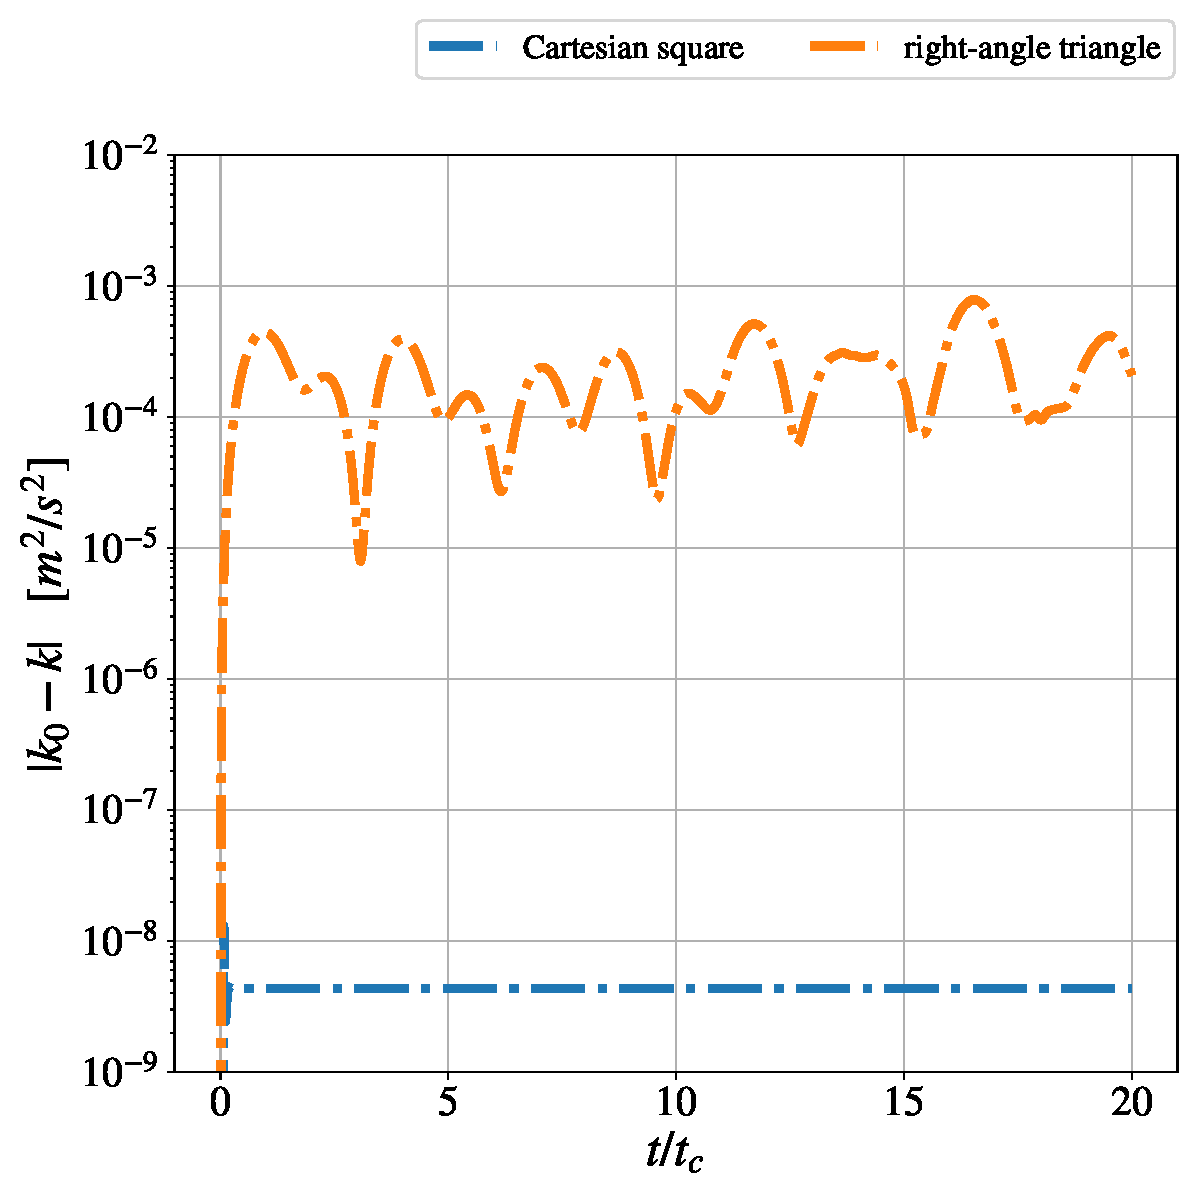
\includegraphics[width=\imgHalfWidth\columnwidth]{TGV2D/inviscid/spaeceFoamCNTGV_regular_inviscid_quadVsRAT_KEevolution_8x8_k_Log.pdf}\label{fig:TGV2D-inv-k}}
\subfloat[advection \& pressure grad. KE transport]{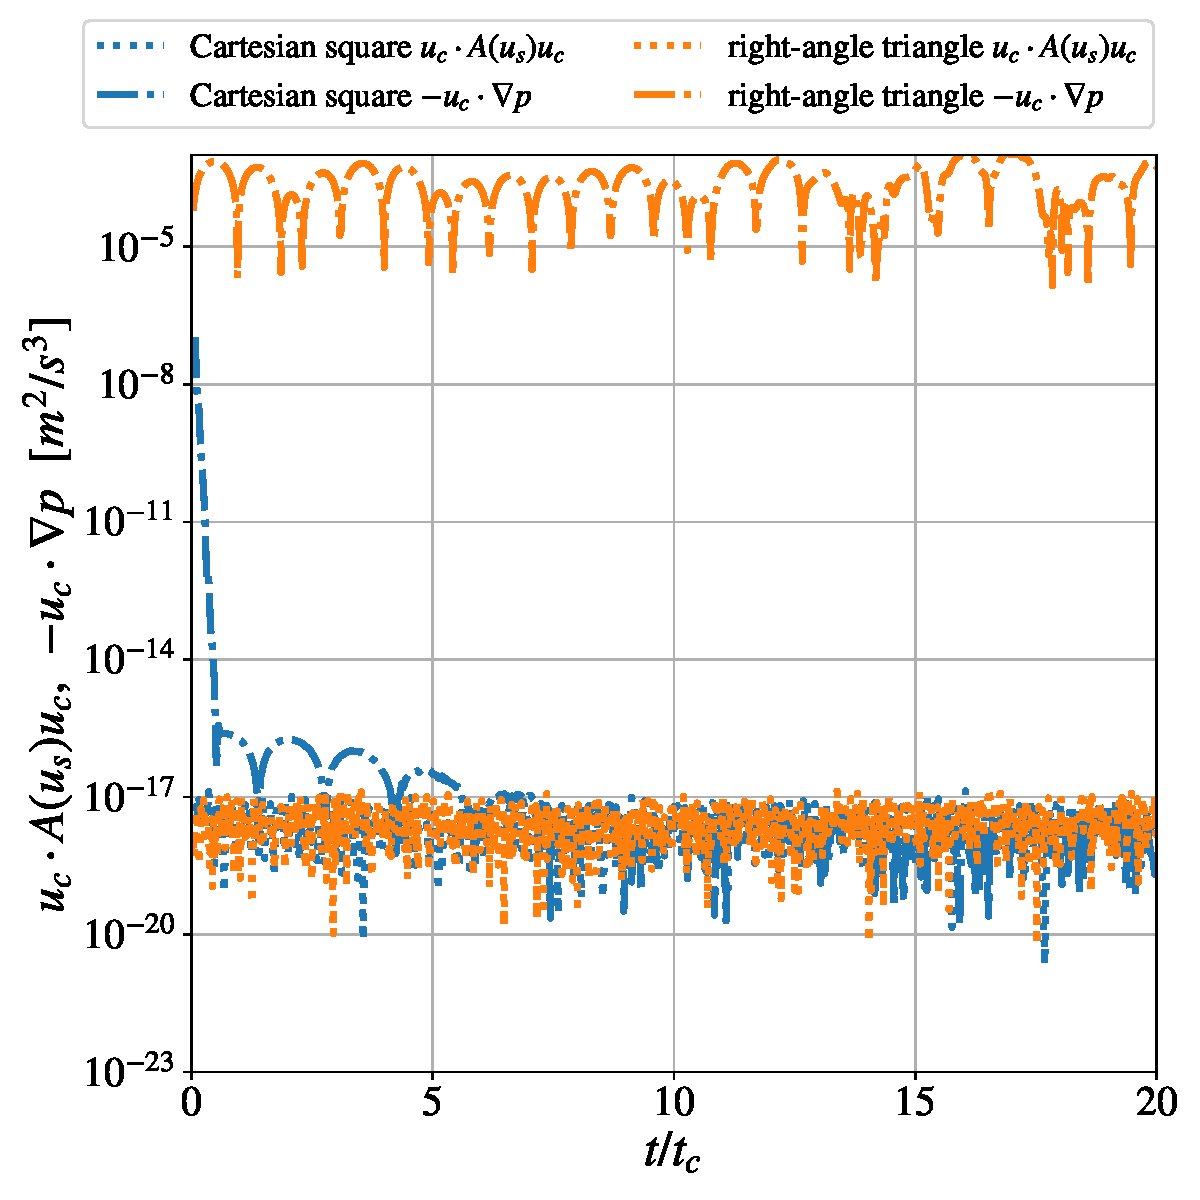
\includegraphics[width=\imgHalfWidth\columnwidth]{TGV2D/inviscid/spaeceFoamCNTGV_regular_inviscid_quadVsRAT_KEcomparison_semiLogY_advection_gradP.pdf}\label{fig:TGV2D-inv-adv}} 
\caption{Inviscid 2D Taylor-Green vortex KE, and advection and pressure gradient KE transport terms evolution comparison between a Cartesian square $65 \times 65$ mesh and a right angle triangle $(65 \times 65)\times 2$ mesh.} 
\label{fig:TGV2D-inv}
\end{figure}

For an inviscid flow $(\nu = 0)$, KE change is compared between a Cartesian square $65 \times 65$ mesh and a right-angle triangulated $(65 \times 65)\times 2$ mesh over 20 characteristic time period (Fig. \ref{fig:TGV2D-inv-k}). KE transport (Eq. \ref{eqn:KE1}) contribution from the advection term $\transDot{\avb{u}_c} \mathbf{A}(\avb{u}_f) {\avb{u}_c} $ and pressure gradient term $\transDot{\avb{u}_c} \mathbf{V}\mathbf{G}_c \avb{p}$ is also compared (Fig. \ref{fig:TGV2D-inv-adv}).

The total KE is fairly constant for both mesh types(Fig. \ref{fig:TGV2D-inv-k}). However, the right-angle triangulated mesh has higher error from initial KE $k_0$ due to a larger difference in collocated and staggered gradient operators arising from unequal control volumes and non-orthogonal correction (see pressure gradient transport term in Fig. \ref{fig:TGV2D-inv-adv}). Contribution from the advection transport term is machine zero for both mesh types.


\subsubsection{3D Taylor-Green vortex}
A 3D Taylor-Green vortex field is initialized in a cubic domain $x, y,z \in [-\pi, \pi]$ with unit characteristic length $L$ and density $\rho_0$, and characteristic velocity $U=0.1$ following the analytical expression
\begin{equation}
\begin{split}
u_0 &=U \sin \left(\frac{x}{L}\right) \cos \left(\frac{y}{L}\right) \sin \left(\frac{z}{L}\right),
\\
v_0 &=-U \cos \left(\frac{x}{L}\right) \sin \left(\frac{y}{L}\right) \sin \left(\frac{z}{L}\right), 
\\
w_0 &=0, 
\\
p_0 &=\frac{\rho_{0} U^{2}}{16} \left[\cos \left(\frac{2 x}{L}\right)+\cos \left(\frac{2 y}{L}\right)\right] \left[\cos \left(\frac{2 z}{L}\right)+2\right].
\end{split}
\end{equation}

In absence of viscosity ($\nu=0$), KE changes is compared among a Cartesian cubic $65 \times 65 \times 65$ mesh, a right-angle triangulated prism $(65 \times 65)\times 2 \times 65$ mesh and a Cartesian non-uniform hexagonal $65 \times 65 \times 65$ mesh, where control volumes are uniform at the center and nodes are clustered in the corner leading to maximum aspect ratio of 5.3. KE is fairly constant over time across all mesh types (Fig. \ref{fig:TGV3D-inv-k}) and the non-uniform hexagonal mesh has the highest error can be attributed to large pressure gradient KE transport error evident in Fig. \ref{fig:TGV3D-inv-adv}. Similar to the 2D case, contribution from the advection KE transport term is machine zero for all cases.

\begin{figure}[!h]
\centering
\subfloat[KE evolution]{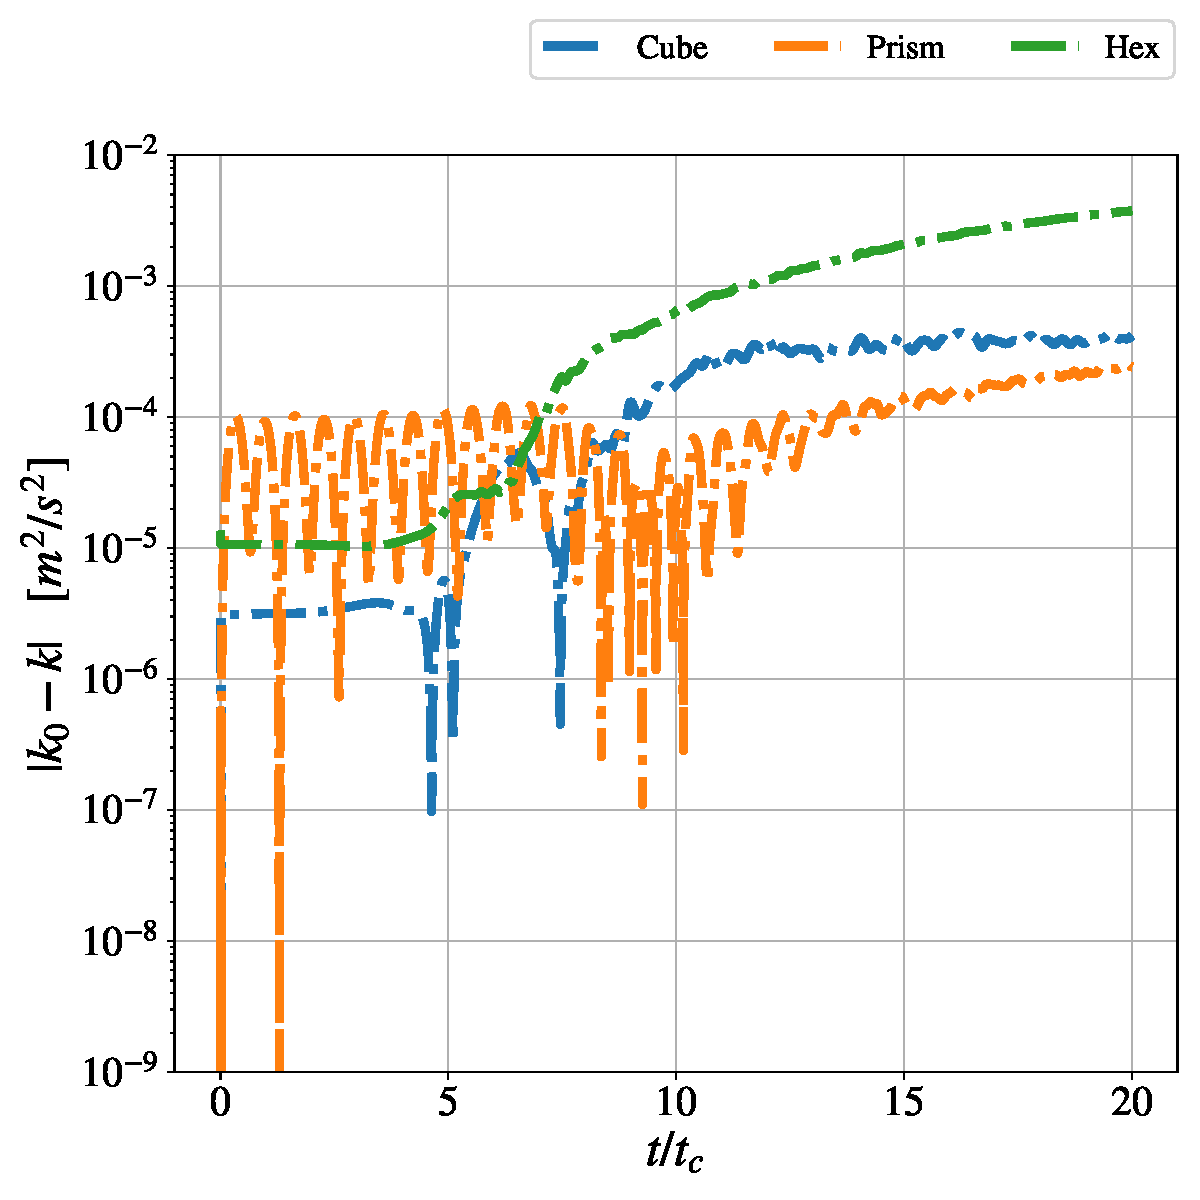
\includegraphics[width=\imgHalfWidth\columnwidth]{TGV3D/inviscid/3Mesh/spaeceFoamCNTGV_inviscid_cubeVsPrismVsHex_KEevolution_8x8_k_Log.pdf}\label{fig:TGV3D-inv-k}}
\subfloat[advection \& pressure grad. KE transport]{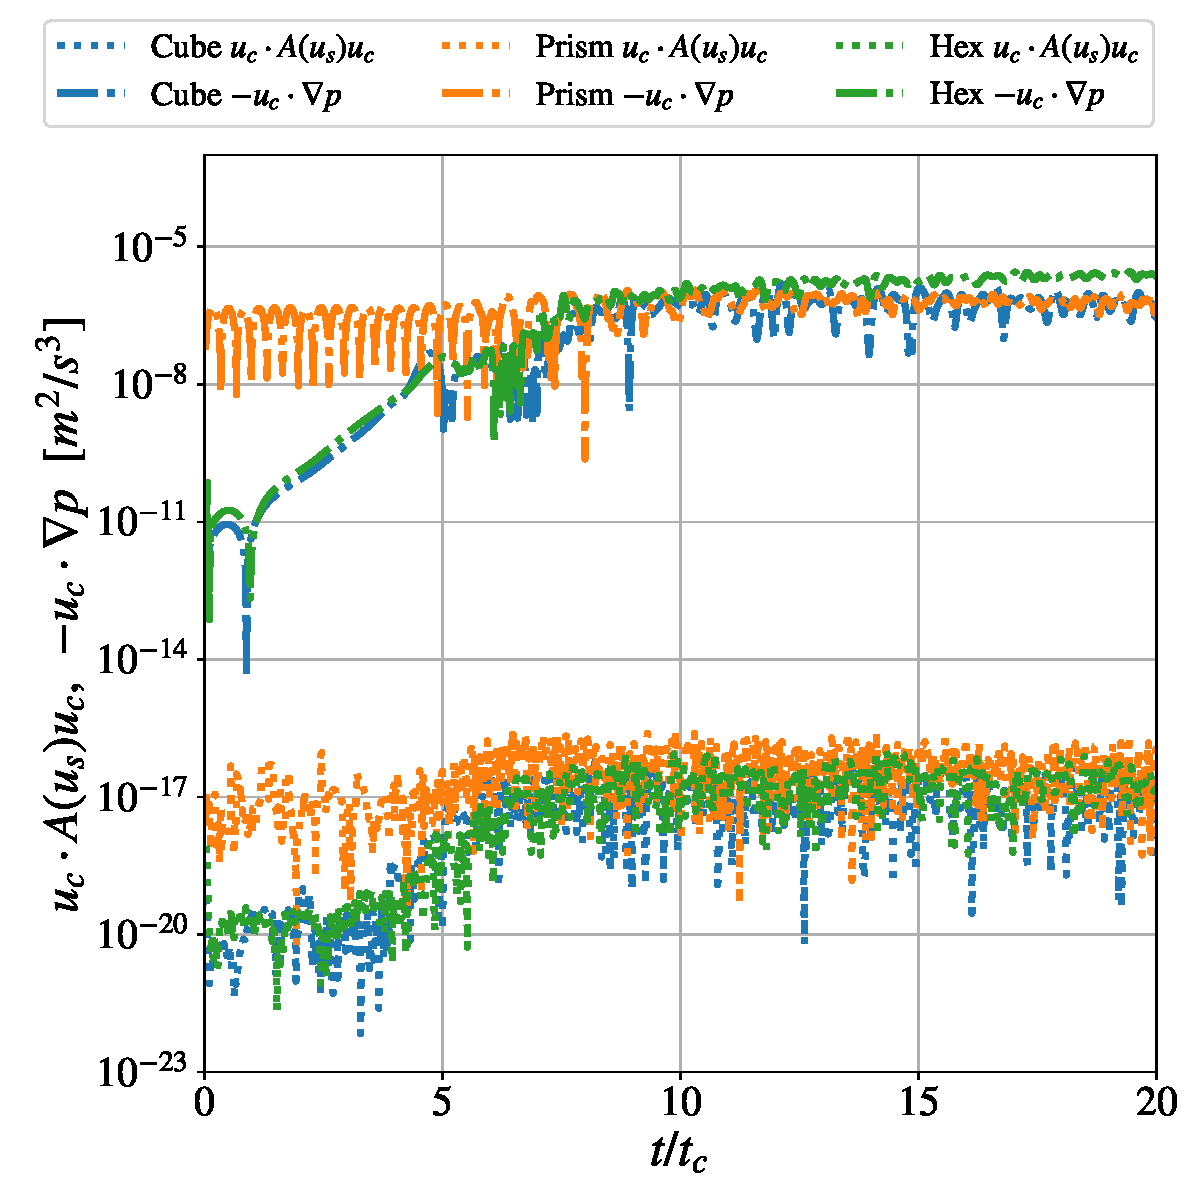
\includegraphics[width=\imgHalfWidth\columnwidth]{TGV3D/inviscid/3Mesh/spaeceFoamCNTGV_inviscid_cubeVsPrismVsHex_KEcomparison_8x8_semiLogY_advection_gradP.pdf}\label{fig:TGV3D-inv-adv}} 
\caption{Inviscid 3D Taylor-Green vortex KE, and advection and pressure gradient KE transport terms evolution comparison among three mesh types.} 
\label{fig:TGV3D-inv}
\end{figure}


To preserve (skew-)symmetry property of the discrete advection, pressure gradient and dissipation operators (Eqs. \eqref{eqn:operatorProperties}, \eqref{eqn:advOpConstraint}, \eqref{eqn:gradOpConstraint} and \eqref{eqn:LaplaceOp} respectively), the importance of using mid-point interpolation scheme is outlined. For the non-uniform Cartesian hexagonal mesh, KE evolution comparison between mid-point and linear interpolation schemes for an inviscid 3D Taylor-Green vortex is illustrated in Fig. \ref{fig:TGV3D-inv-hex}. Use of linear interpolation scheme leads to unbounded growth of the advection KE transport term and ultimately, made the linear system unstable. In contrast, the mid-point interpolation scheme kept it to machine zero and ensured solver stability.

\begin{figure}[!h]
\centering
\subfloat[KE evolution]{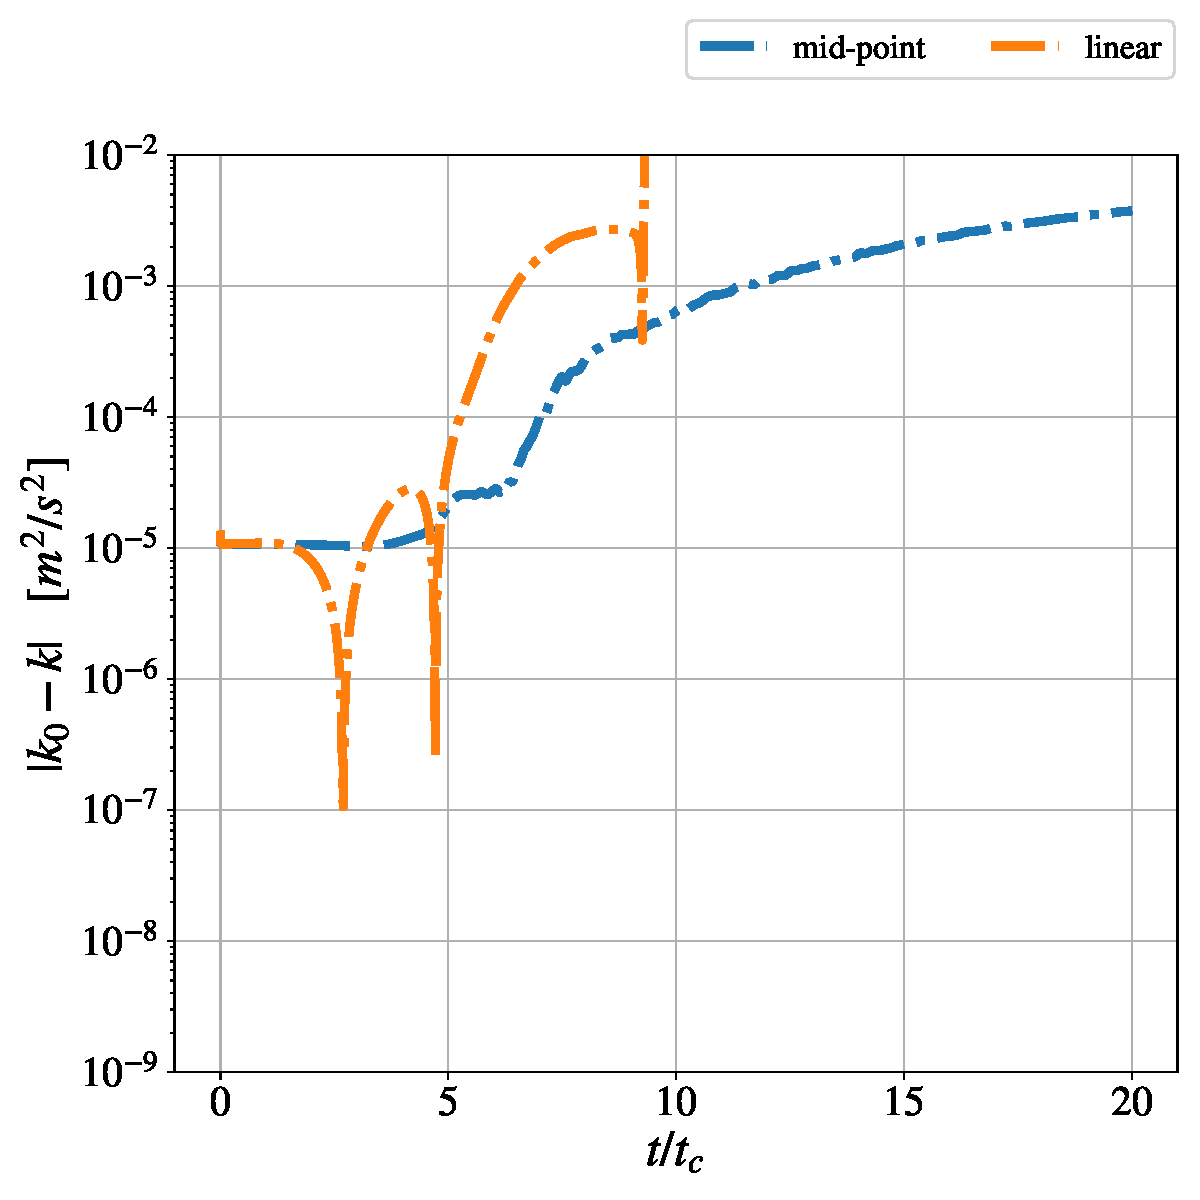
\includegraphics[width=\imgHalfWidth\columnwidth]{TGV3D/inviscid/midpointVsLinear/spaeceFoamCNTGV_inviscid_midpointVsLinear_KEevolution_8x8_k_Log.pdf}\label{fig:TGV3D-inv-hex-k}}
\subfloat[advection \& pressure grad. KE transport]{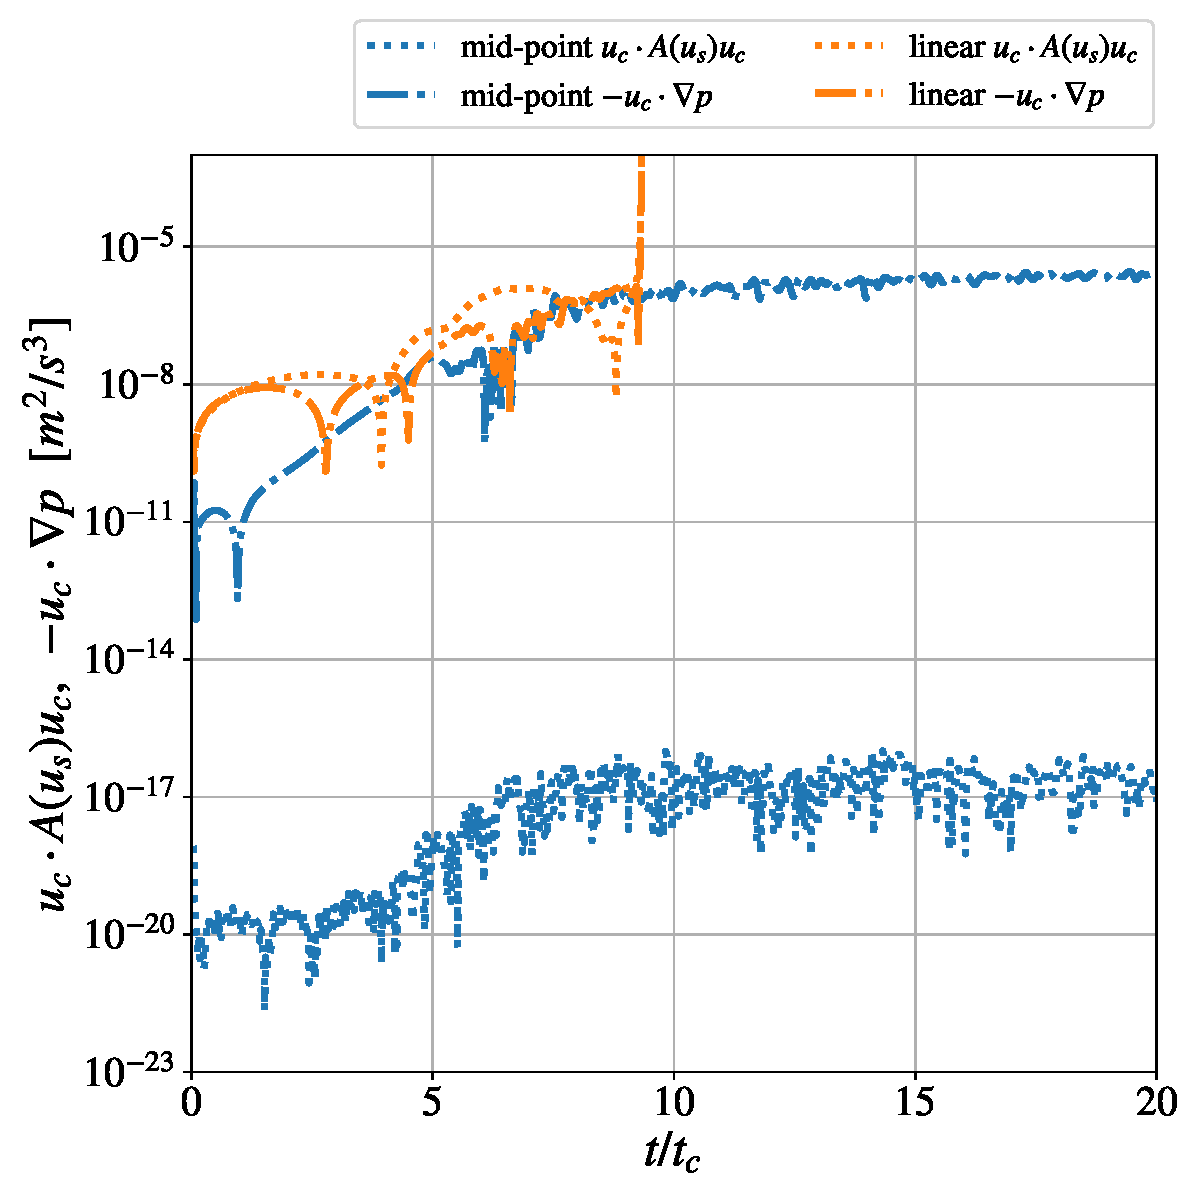
\includegraphics[width=\imgHalfWidth\columnwidth]{TGV3D/inviscid/midpointVsLinear/spaeceFoamCNTGV_inviscid_midpointVsLinear_KEcomparison_8x8_semiLogY_advection_gradP.pdf}\label{fig:TGV3D-inv-hex-adv}} 
\caption{Inviscid 3D Taylor-Green vortex KE, and advection and pressure gradient KE transport terms evolution comparison between midpoint and linear interpolation schemes for the Cartesian non-uniform hexagonal $65 \times 65 \times 65$ mesh.} 
\label{fig:TGV3D-inv-hex}
\end{figure}



\clearpage
\subsubsection{Influence of A6 regularization}
\label{sec:A6KEconserv}

In Sec. \ref{sec:advReg}, we have identified that the in-exact shift-operators lead to higher divergence error for the residual-filtered face-velocity $\avbPrime{u_f}$, which ultimately break KE conservation. In Fig. \ref{fig:TGV3D-inv-A6}, KE evolution and KE transport contribution from the advection and pressure gradient terms are compared among the \spaece, \spaeceA and \spaeceAdivFree algorithms in a Cartesian non-uniform hexagonal $65 \times 65 \times 65$ mesh. The \spaeceAdivFree and \spaece algorithms conserve KE energy and the advection term is close to machine zero. The KE for the \spaeceA algorithm gradually diverges (Fig. \ref{fig:TGV3D-inv-A6-k}) dueto accumulation of large, non-zero advection transport term (Fig. \ref{fig:TGV3D-inv-A6-adv}). Overall, in a collocated mesh formulation the \spaeceAdivFree maintains KE conservation, while \spaeceA introduce non-zero advection KE transport term.

\begin{figure}[!h]
\centering
\subfloat[KE evolution]{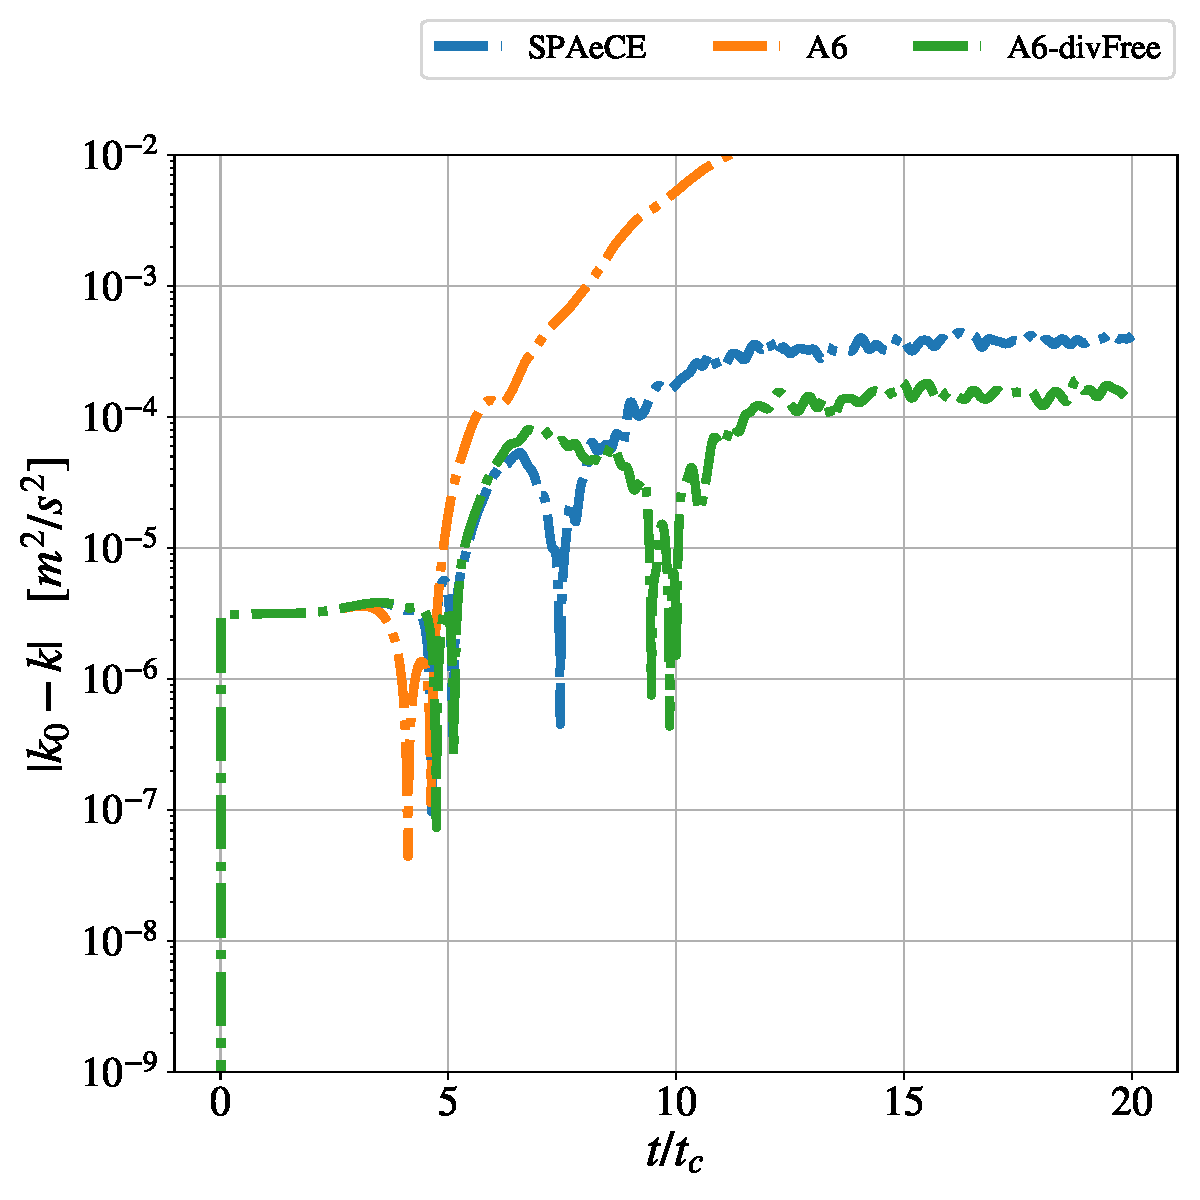
\includegraphics[width=\imgHalfWidth\columnwidth]{TGV3D/inviscid/A6phiResCorrVsA6phiDivFree/spaeceFoamCNTGV_inviscid_A6phiCorrvsA6divFree_KEevolution_8x8_k_Log.pdf}\label{fig:TGV3D-inv-A6-k}}
\subfloat[advection \& pressure grad. KE transport]{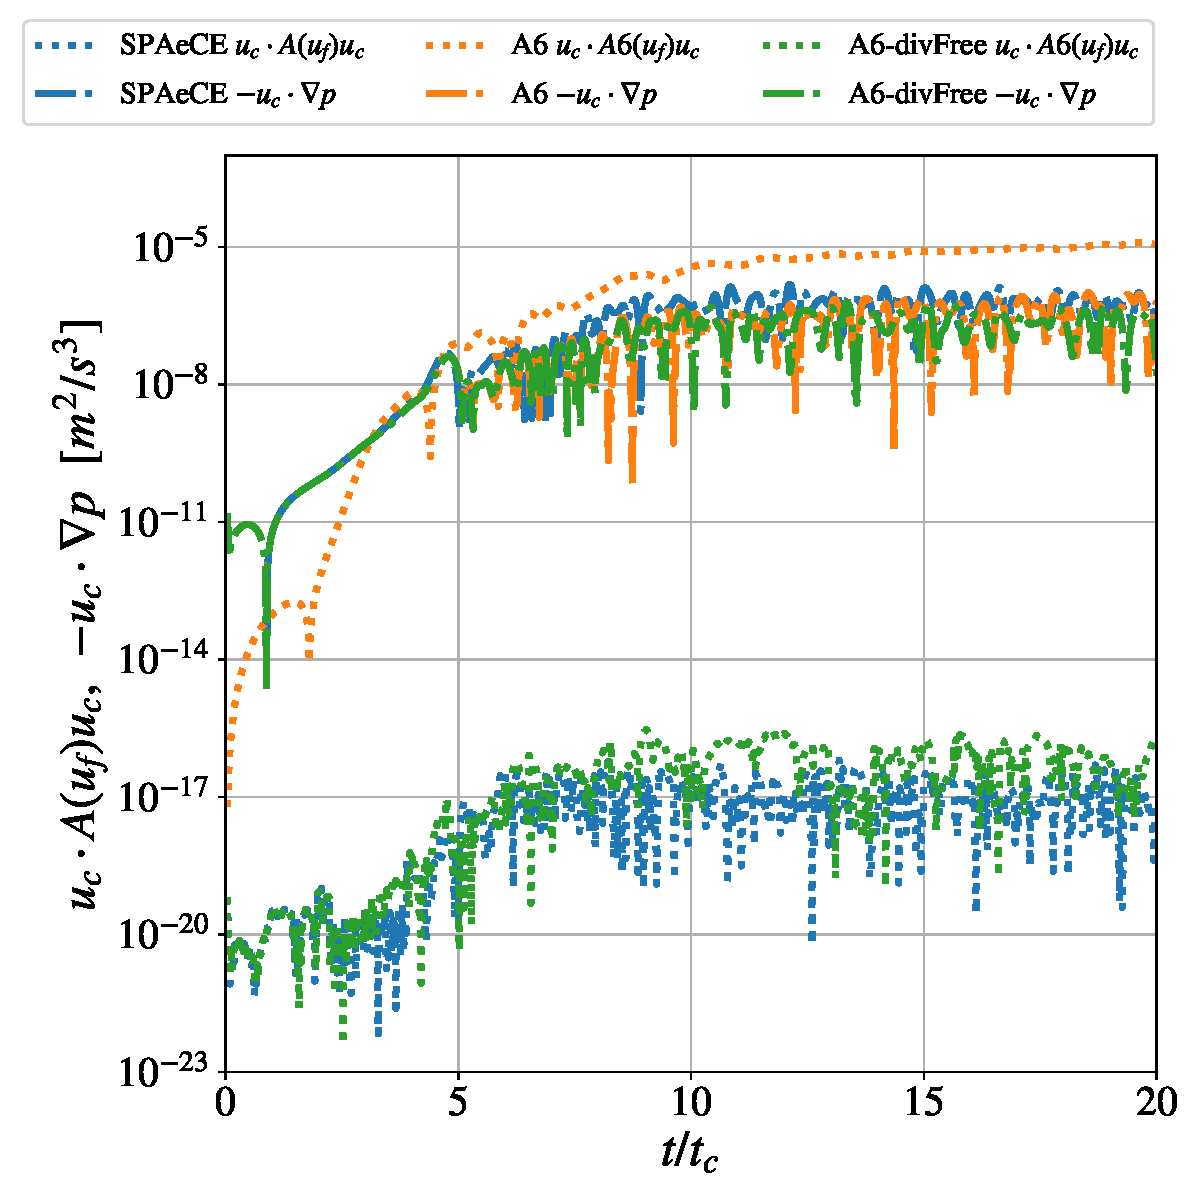
\includegraphics[width=\imgHalfWidth\columnwidth]{TGV3D/inviscid/A6phiResCorrVsA6phiDivFree/spaeceFoamCNTGV_inviscid_A6phiCorrvsA6divFreeKEcomparison_8x8_semiLogY_advection_gradP.pdf}\label{fig:TGV3D-inv-A6-adv}} 
\caption{Inviscid 3D Taylor-Green vortex KE, and advection and pressure gradient KE transport terms evolution comparison among the \spaece, \spaeceA and \spaeceAdivFree algorithms in a Cartesian non-uniform hexagonal $65 \times 65 \times 65$ mesh} 
\label{fig:TGV3D-inv-A6}
\end{figure}







\clearpage
\newpage
\subsection{Order of convergence}
\label{sec:orderOfCon}
\subsubsection{Order of convergence without Rhie-Chow correction}
A viscous 2D Taylor-Green vortex case, applying same domain and initialization as the invicisd case described in section \ref{sec:TGV2d-inv}, but with $Re=1\times10^3,\quad \nu = 1\times10^{-3}$ which dictates the flow as \textit{laminar}. The discrete differential operators are discretized with a Crank-Nicolson temporal scheme and 2nd order central difference spatial schemes with mid-point interpolation. The linear systems are solved for a tolerance of $1\times10^{-15}$. Flow is simulated for $t/t_c = 1.12$ time for all cases and error norms are reported in Fig. \ref{fig:TGV2D-Cart1000-spaece}. 

\begin{figure}[!h]
\centering
\subfloat[Temporal convergence ($257 \times 257$ mesh)]{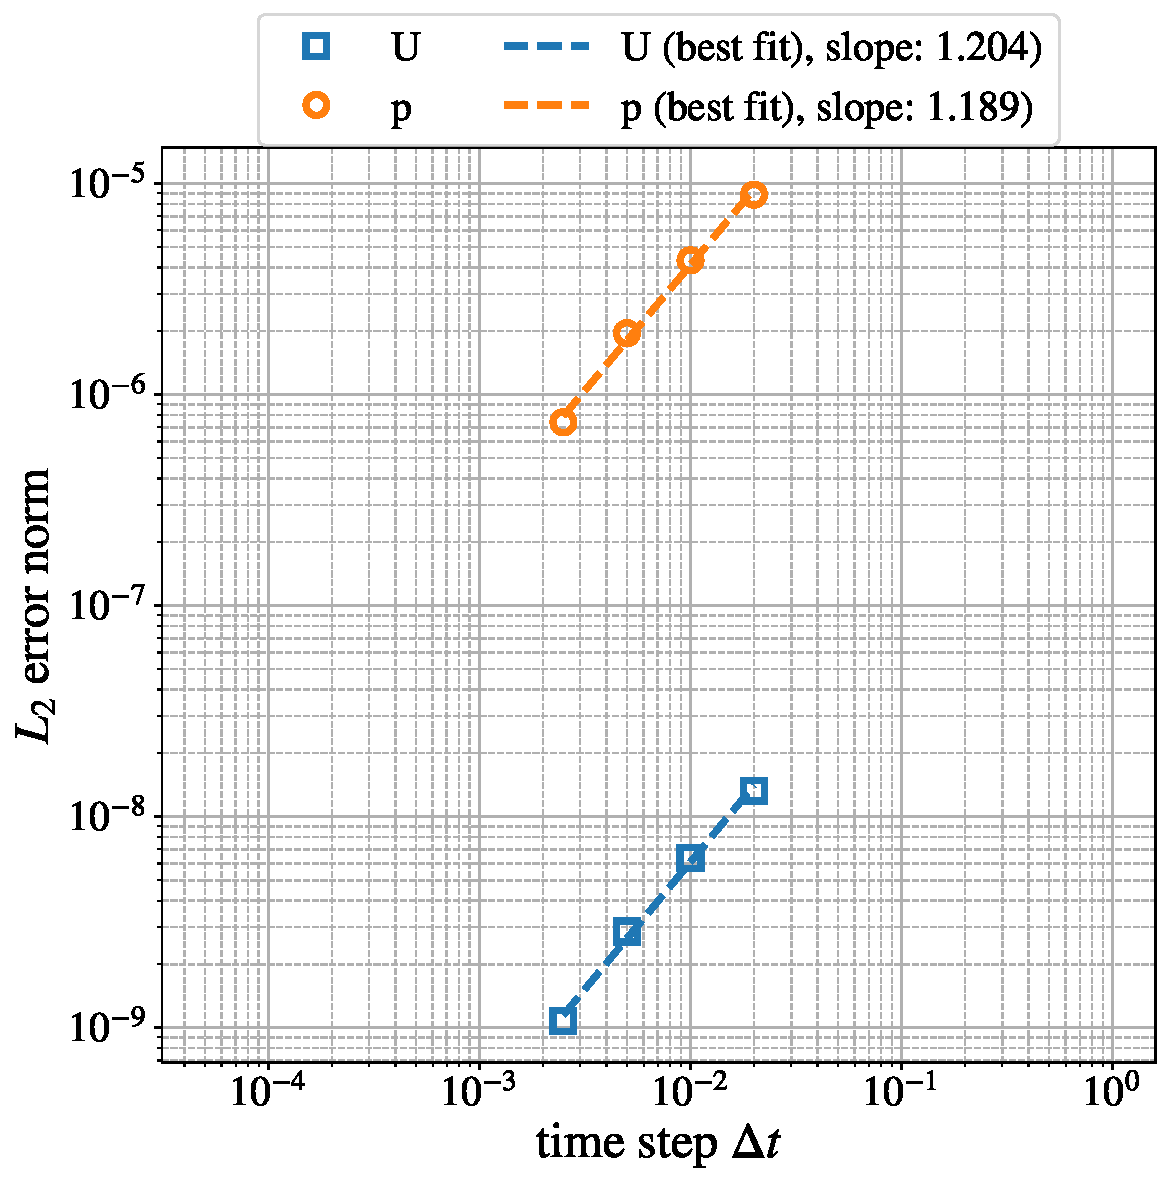
\includegraphics[width=\imgHalfWidth\columnwidth]{TGV2D/Re1000/Cartesian/spaeceFoamCNTGV/regular/temporalConvergence/spaeceFoamCNTGV_Re1000_regular_257x257_log_2ndErrorNorm_refTime_1_12.pdf}\label{fig:TGV2D-Cart1000-spaece-tempCon}}
\subfloat[Spatial convergence (time step $0.001s$)]{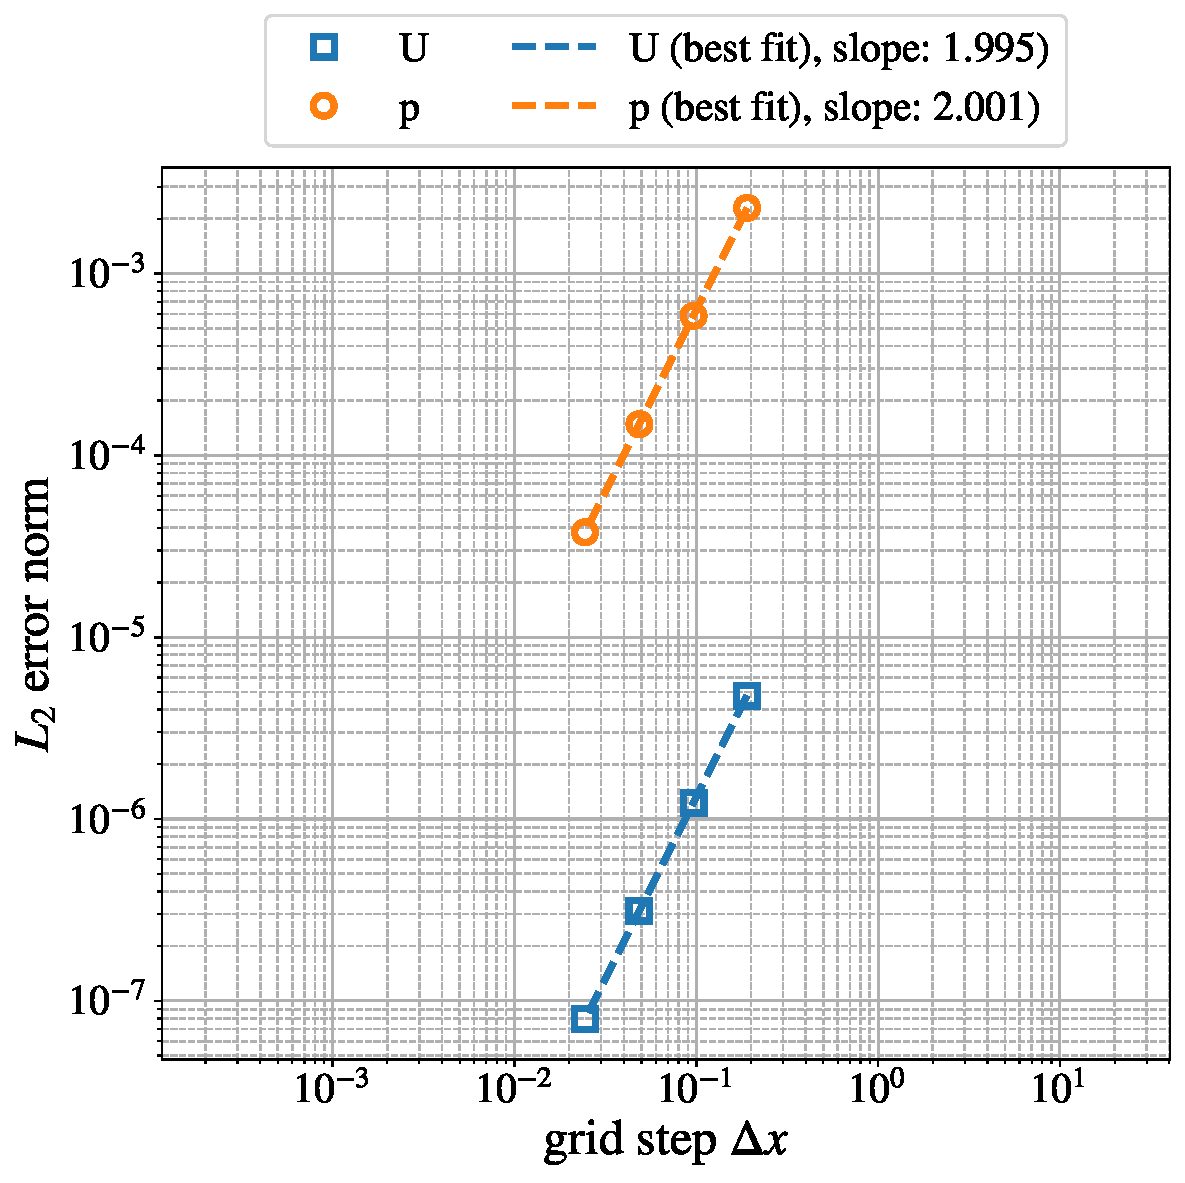
\includegraphics[width=\imgHalfWidth\columnwidth]{TGV2D/Re1000/Cartesian/spaeceFoamCNTGV/regular/gridConvergence/spaeceFoamCNTGV_Re1000_regular_1e-3_2ndErrorNorm.pdf}\label{fig:TGV2D-Cart1000-spaece-spatCon}} 
\caption{Temporal and spatial error norms convergence of the \spaece algorithm for a 2D Taylor-Green vortex with $Re=1\times10^3$ simulated in Cartesian square meshes} 
\label{fig:TGV2D-Cart1000-spaece}
\end{figure}

To determine the temporal convergence rate, flow is simulated on a Cartesian square $257 \times 257$ mesh for a series of time steps $0.02, 0.01, 0.005 $ and $0.0025$. To isolate the spatial discretization error, a reference simulation is performed with time step $1\times10^{-3}$ and reference error norms are subtracted from error norms of larger time steps. The temporal convergence for $L_2$ error norms is 1st order accurate (Fig. \ref{fig:TGV2D-Cart1000-spaece-tempCon}). Although, the Crank-Nicolson scheme is 2nd order accurate, the inherent splitting error of the \spaece algorithm is first order accurate and when combined with 2nd order temporal schemes delivered 1st order temporal convergence only. The pressure error norms are about $1\times10^3$ times higher than the velocity error norms.

Spatial error convergence rate is determined by simulating the flow in four Cartesian square meshes: $33 \times 33$, $65 \times 65$, $127 \times 127$ and $257 \times 257$. To keep the temporal discretization error minimal, a small time-step $1\times10^{-3}s$ is used for all cases. The spatial convergence rate for $L_2$ error norms is 2nd order accurate (Fig. \ref{fig:TGV2D-Cart1000-spaece-spatCon}) and the pressure error norms are approximately $300$ times higher than the velocity error norms. The $L_\infty$ error norms are not reported, but has the same temporal and spatial convergence order as the $L_2$ error norms. 


\subsubsection{Order of convergence with Rhie-Chow correction}
\label{sec:OoC-RC}
To avoid checkerboard like pattern, simulations are performed with Rhie-Chow correction\cite{rhie1983} for face-normal velocity (Eq. \eqref{eqn:updateUfRC}). Fig. \ref{fig:TGV2D-Cart1000-spaeceRC} illustrates the temporal and spatial error convergence for the \spaece algorithm with Rhie-Chow correction (\spaeceRC) evaluated for the same 2D Taylor-Green vortex of $Re\,1\times10^3$ case.
\begin{figure}[!h]
\centering
\subfloat[Temporal convergence]{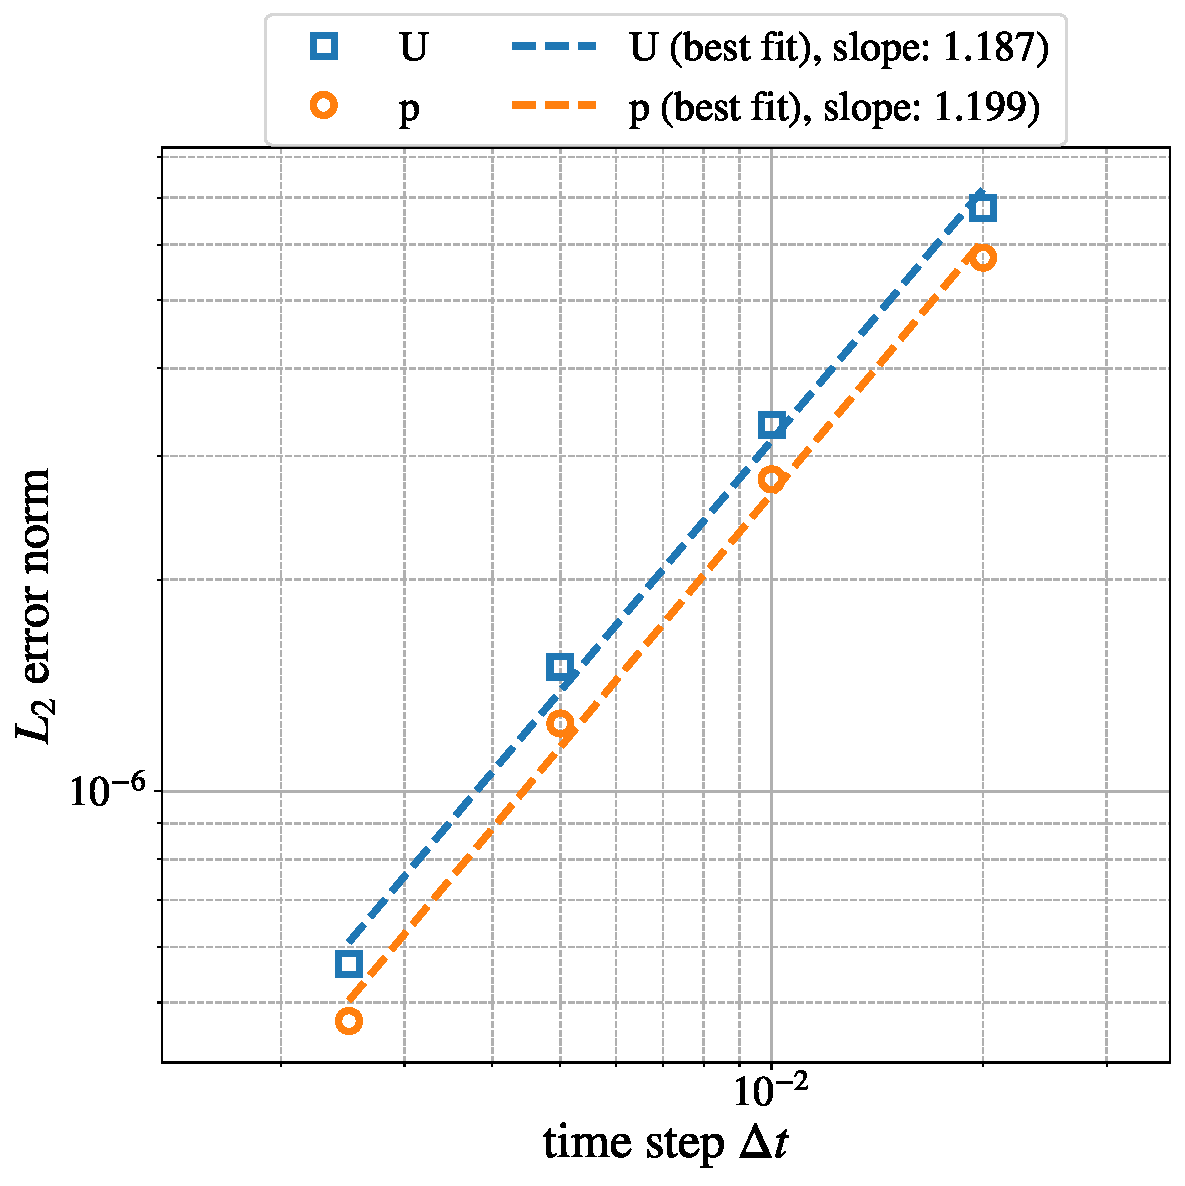
\includegraphics[width=\imgHalfWidth\columnwidth]{TGV2D/Re1000/Cartesian/spaeceFoamCNTGV/regularRC/temporalConvergence/spaeceFoamCNTGV_Re1000_regularRC_257x257_log_2ndErrorNorm_refTime_1_12.pdf}\label{fig:TGV2D-Cart1000-spaeceRC-tempCon}}
\subfloat[Spatial convergence]{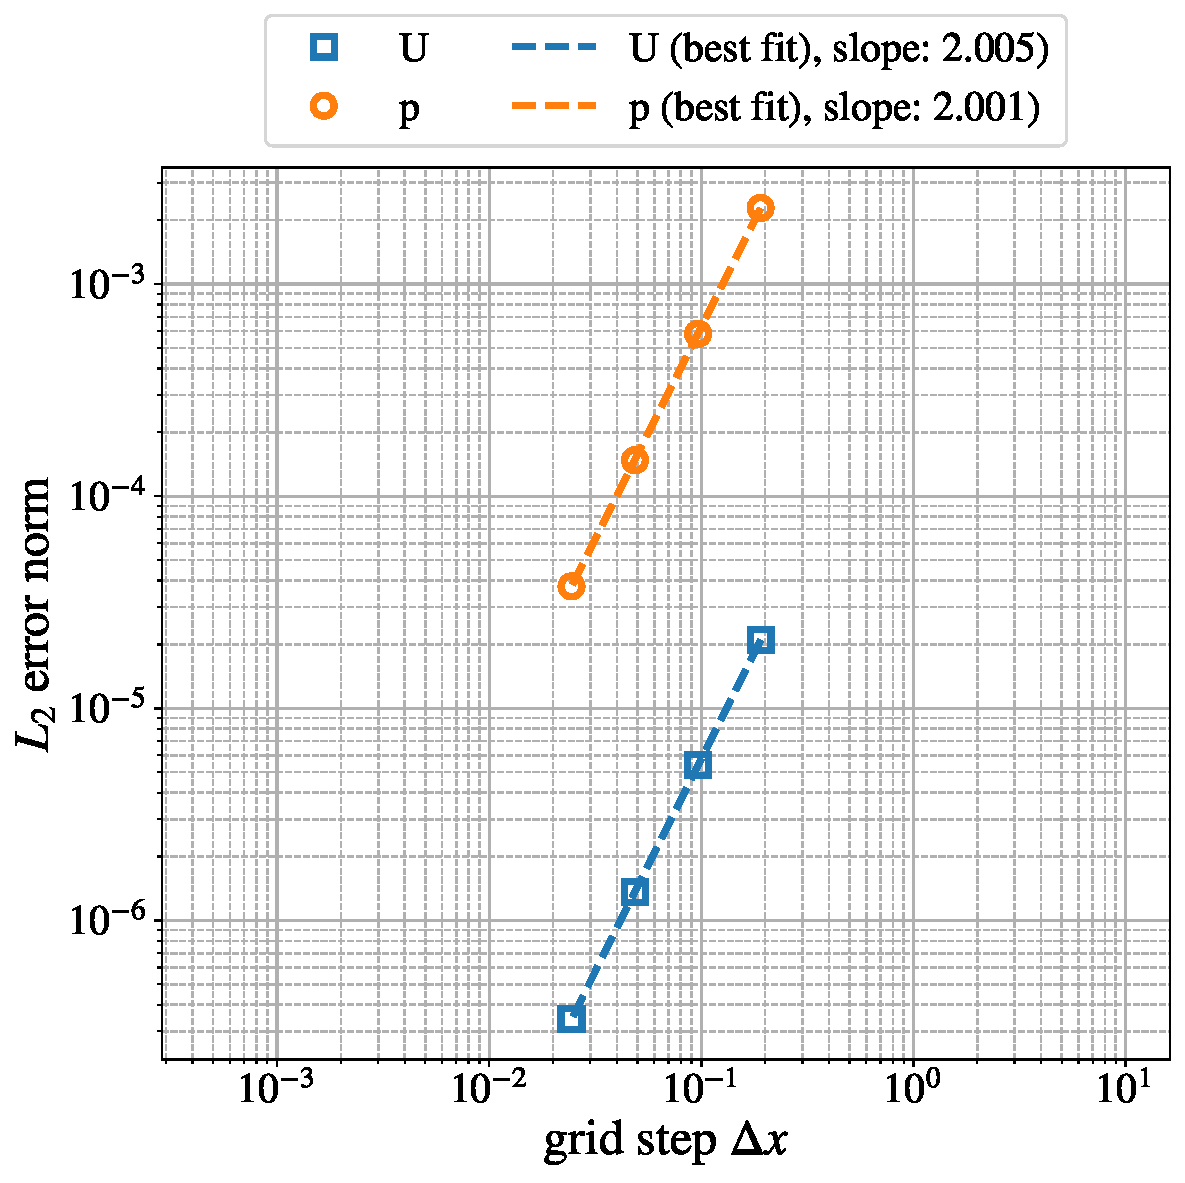
\includegraphics[width=\imgHalfWidth\columnwidth]{TGV2D/Re1000/Cartesian/spaeceFoamCNTGV/regularRC/gridConvergence/spaeceFoamCNTGV_Re1000_regularRC_1e-3_2ndErrorNorm.pdf}\label{fig:TGV2D-Cart1000-spaeceRC-spatCon}} 
\caption{Temporal and spatial error norms convergence of the \spaeceRC algorithm for a 2D Taylor-Green vortex with $Re\,1\times10^3$ simulated in Cartesian square meshes} 
\label{fig:TGV2D-Cart1000-spaeceRC}
\end{figure}

The temporal error convergence remained 1st order accurate, while the velocity error magnitudes are increased to pressure error levels (Fig. \ref{fig:TGV2D-Cart1000-spaeceRC-tempCon}). The spatial error convergence rate is also maintained 2nd order convergence with increased velocity error (Fig. \ref{fig:TGV2D-Cart1000-spaeceRC-spatCon}). The $L_\infty$ error norms produced same order of convergence as the $L_2$ error norms, thus not reported.
%

The \piso algorithm implementation in OpenFOAM \cite{weller1998} has an indirect implementation of the Rhie-Chow correction, where the staggered velocity is updated excluding the pressure gradient. It requires significant change in staggered velocity update (Eq. \eqref{eqn:updateUfRC}), Poisson pressure solve (Eq. \eqref{eqn:poissonPressure}) and velocity correction (Eq. \eqref{eqn:updateFaceVel}) equations: 
\begin{align}
\begin{split}
\text{Update face-normal velocity: } & 
\avb{u}_f^{n+1, *} = \shiftCS \left[\mathcal{A_F}^{-1} ( \mathcal{H} + \mathcal{S}) \right] \cdot \faceUnitNormal,
\\
\text{Poisson pressure solve: } & \mathcal{L} \mathcal{A_F}^{-1}  \, \avb{p}_c = \mathcal{M} \avb{u}_f^{n+1,*},
\\
\text{Correct face-normal velocity: } & \avb{u}_f^{n+1} = \avb{u}_f^{n+1, *} - \mathcal{A_F}^{-1} \, \mathcal{G_F}\avb{p}_c .
\end{split}
\label{eqn:openfoamPiso}
\end{align}

\begin{figure}[!h]
\centering
\subfloat[temporal convergence]{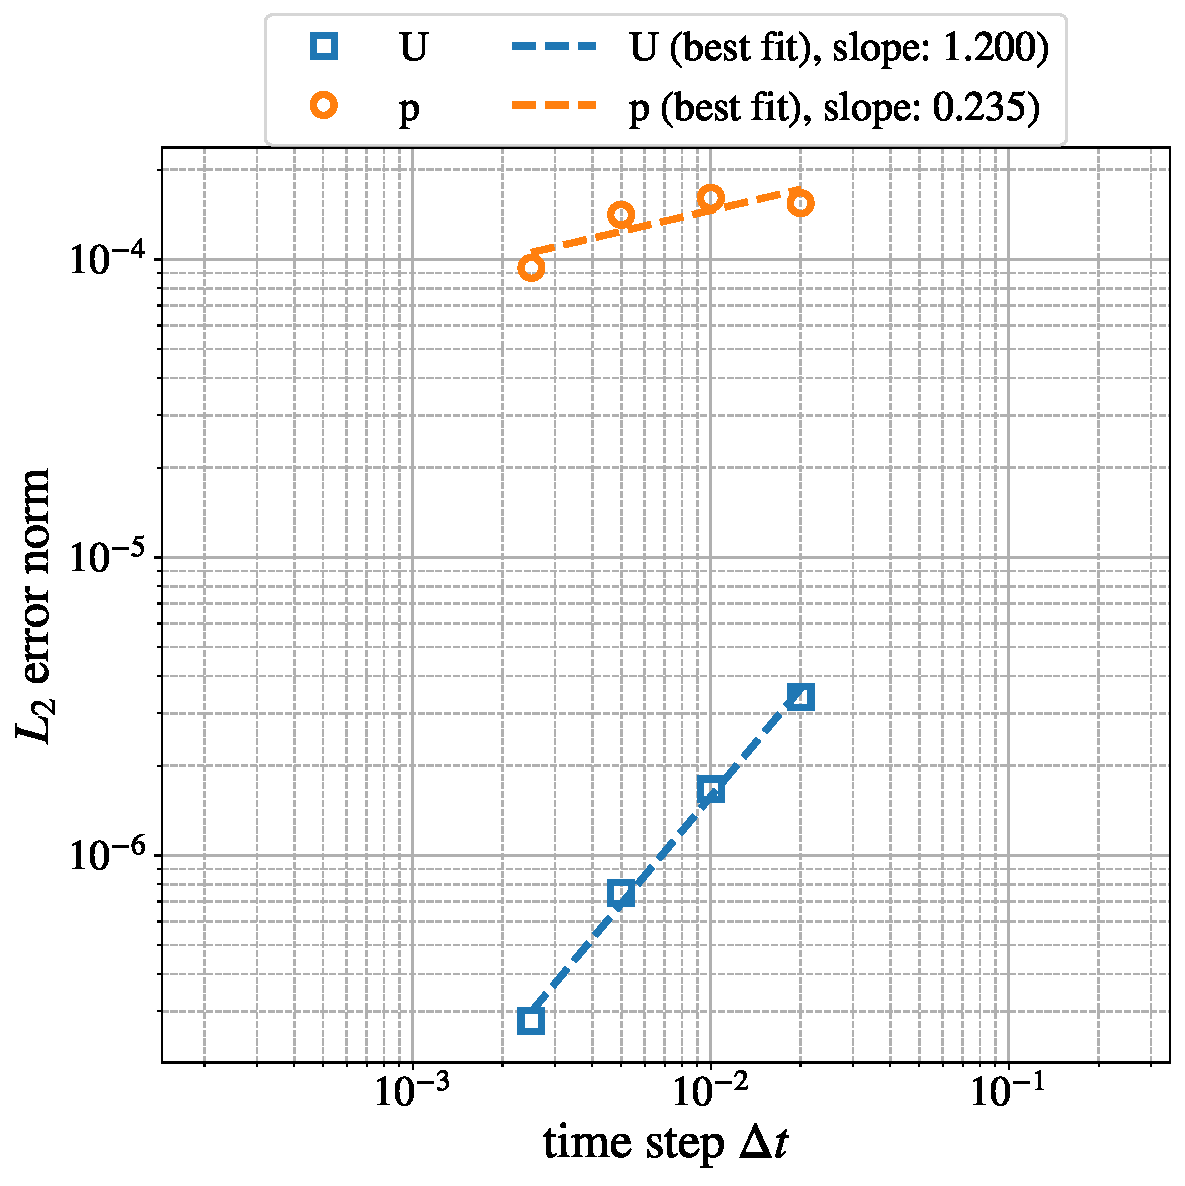
\includegraphics[width=\imgHalfWidth\columnwidth]{TGV2D/Re1000/Cartesian/pisoFoamwoDdtCorr/CN1/temporalConvergence/pisoFoamwoDdtCorr_Re1000_CN1_257x257_log_2ndErrorNorm_refTime_1_12.pdf}\label{fig:TGV2D-Cart1000-piso-tempCon}}
\subfloat[spatial convergence]{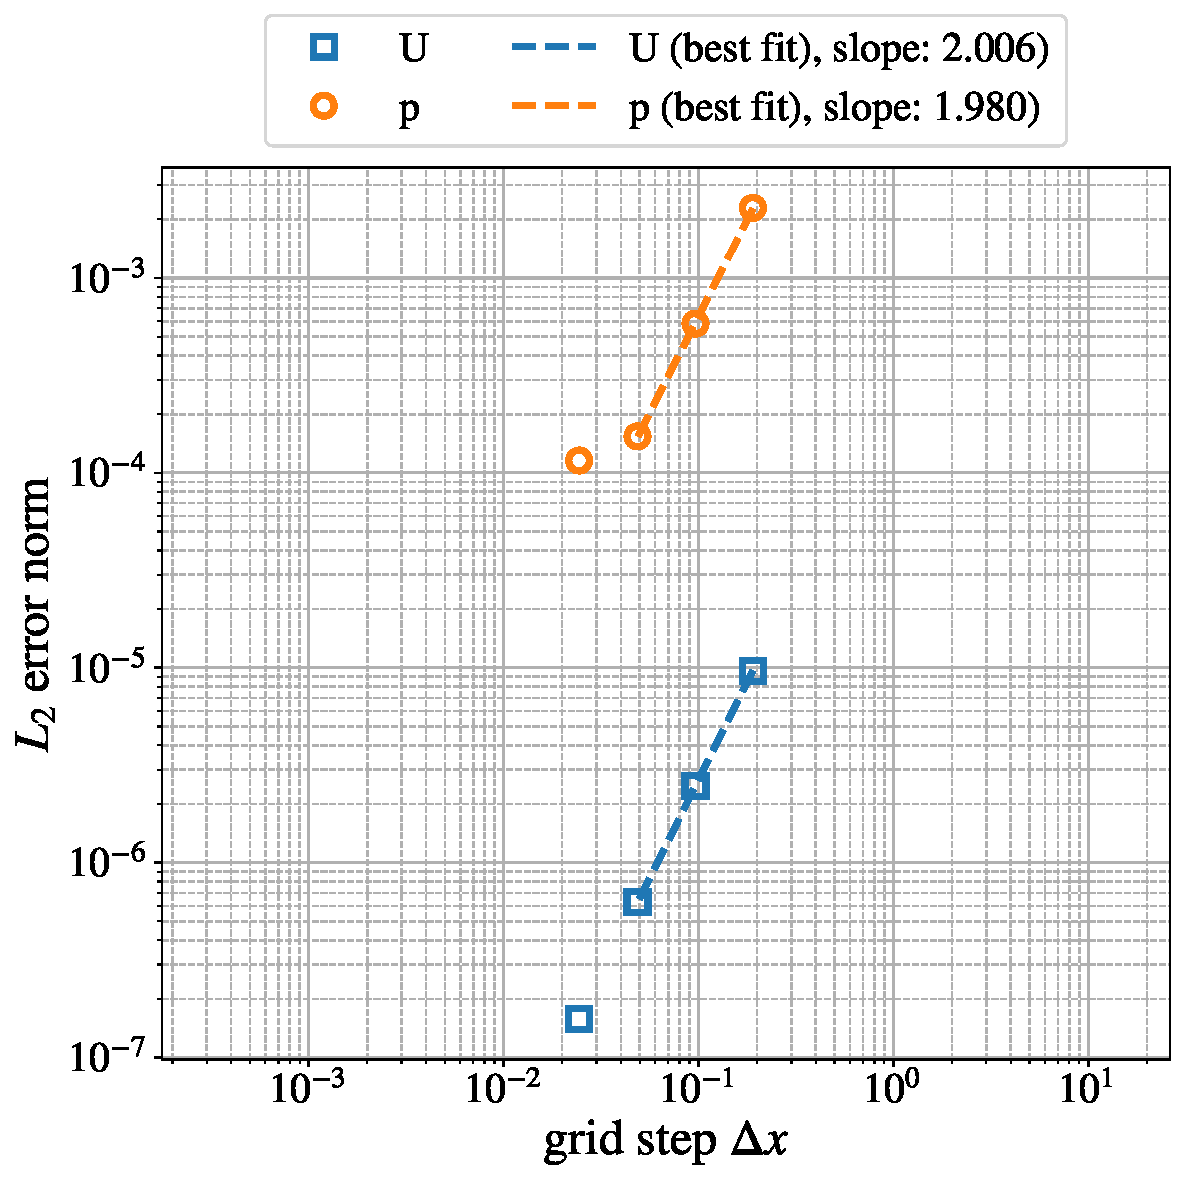
\includegraphics[width=\imgHalfWidth\columnwidth]{TGV2D/Re1000/Cartesian/pisoFoamwoDdtCorr/CN1/gridConvergence/pisoFoamwoDdtCorr_Re1000_CN1_1e-3_2ndErrorNorm.pdf}\label{fig:TGV2D-Cart1000-piso-spatCon}} 
\caption{Temporal and spatial error norms convergence of the OpenFOAM \piso algorithm (without  Rhie-Chow correction for time step) for a 2D Taylor-Green vortex with $Re\,1\times10^3$ simulated in Cartesian square meshes.} 
\label{fig:TGV2D-Cart1000-piso}
\end{figure}

Following the \spaeceRC algorithm validation, temporal and spatial error convergence for OpenFOAM \piso algorithm implementation (with two pressure solve iterations and without Rhie-Chow correction for time-step \footnote{The authors observed that the Rhie-Chow correction for time-step introduces excessive artificial dissipation, often appeared as the largest source of dissipation. To facilitate comparison with the \spaeceRC and \spaeceARC algorithms, the  Rhie-Chow correction for time-step is excluded from the OpenFOAM \piso algorithm.}) is illustrated in Fig. \ref{fig:TGV2D-Cart1000-piso}. The temporal convergence for velocity is first order, but pressure is close to zeroth order(Fig. \ref{fig:TGV2D-Cart1000-piso-tempCon}). Both the velocity and pressure fields demonstrated a 2nd order convergence for spatial error norms (Fig. \ref{fig:TGV2D-Cart1000-piso-spatCon}). The $L_\infty$ error norms of the \piso algorithm delivered same order of convergence as the $L_2$ error norms.

\begin{figure}[!ht]
\centering
\subfloat[$L_2$ error norm]{\includegraphics[width=\imgHalfWidth\columnwidth]{TGV2D/Re1000/Cartesian/ErrorNormComp_2nd.pdf}\label{fig:TGV2D-Cart1000-CFL-2nd}}
\subfloat[$L_\infty$ error norm]{\includegraphics[width=\imgHalfWidth\columnwidth]{TGV2D/Re1000/Cartesian/ErrorNormComp_Inf.pdf}\label{fig:TGV2D-Cart1000-CFL-inf}} 
\caption{Order of convergence comparison for across CFL numbers for \spaece, \spaeceRC and \piso algorithms in Cartesian square mesh} 
\label{fig:TGV2D-Cart1000-CFL}
\end{figure}

The isolated temporal and spatial error order of convergence are important indicators of any algorithm. However in practice, fluid flow problems are often solved at a certain CFL number\cite{courant1928, courant1967} limit and in such cases, the mixed order of convergence is also import to the user. 2D Taylor-Green vortex at $Re\, 1\times10^3$ is simulated in four Cartesian square meshes: $33 \times 33$, $65 \times 65$, $127 \times 127$ and $257 \times 257$. Times steps are adjusted for each mesh to simulate the cases in a series of four CFL numbers: $0.1, \, 0.2,\, 0.4$ and $0.8$. The order of convergence for the \spaece, \spaeceRC and \piso algorithms are reported in Fig. \ref{fig:TGV2D-Cart1000-CFL}. 
%(i.e. $4\times 4 = 16$ simulations)

The \spaece algorithm demonstrated 2nd order error convergence for both velocity and pressure fields with slight decrease at high CFL numbers. Application of  Rhie-Chow correction increased velocity error convergence rate to 3rd order for both \spaeceRC and \piso algorithms. The \spaeceRC algorithm delivered 2nd order error convergence for pressure at CFL $0.1$ and proportionally decreased to 1.58th order for CFL $0.8$. On the other hand, the \piso algorithm achieved 1.2th order of convergence for pressure, which gradually increased to 1.75th order at CFL $0.8$. 
Overall, at $CFL < 0.5 $ the \spaeceRC delivers better pressure error convergence and at $CFL > 0.5$ both of the \spaeceRC and \piso algorithms provide similar near 2nd order error convergence.


%\clearpage
\subsubsection{Order of convergence in non-orthogonal mesh}
Non-orthogonality can bring significant change in order of convergence of any algorithm. The laminar 2D Taylor-Green vortex ($Re\, 1\times10^3$) is simulated in a series of mesh where each square is split into two right-angle triangles (i.e. each triangle has two non-orthogonal faces). Thus, any Cartesian square $N \times N$ mesh is converted into right-angle triangulated $(N \times N) \times 2$ mesh.

\begin{figure}[!h]
\centering
\subfloat[$L_2$ error norm]{\includegraphics[width=\imgHalfWidth\columnwidth]{TGV2D/Re1000/rightAnglePrism/ErrorNormComp_2nd.pdf}\label{fig:TGV2D-RAT1000-CFL-2nd}}
\subfloat[$L_\infty$ error norm]{\includegraphics[width=\imgHalfWidth\columnwidth]{TGV2D/Re1000/rightAnglePrism/ErrorNormComp_Inf.pdf}\label{fig:TGV2D-RAT1000-CFL-inf}} 
\caption{Order of convergence comparison for across CFL numbers for \spaece, \spaeceRC and \piso algorithms in right-angle triangulated mesh} 
\label{fig:TGV2D-RAT1000-CFL}
\end{figure}

Similar to the study on Cartesian square meshes (Sec. \ref{sec:OoC-RC}), the order of error convergence across multiple CFL numbers for right-angle triangulated meshes is reported in Fig. \ref{fig:TGV2D-RAT1000-CFL}. The \spaece algorithm provided inconsistent order of convergence, emphasizing the importance of Rhie-Chow correction. The \spaeceRC and \piso algorithms both provided near-identical results. When compared to the Cartesian square mesh results, the order of convergence for velocity errors dropped from 3rd order to 2.6th order, and the pressure errors are slightly increased above 2nd order. 

%\clearpage
%\newpage
\subsection{Minimize artificial dissipation}
\label{sec:minimizeArtificialDissipation}
In accordance with KE conservation for inviscid flow (Sec. \ref{sec:inviscidKE}), there shall not be any artificial dissipation in a viscous flow simulation, i.e. the molecular and turbulence dissipative terms shall be the sole source KE decay. 

A LES of 3D Taylor-Green vortex with $Re = 5\times10^3$ is simulated with the \spaece algorithm for a Cartesian cubic $65 \times 65 \times 65$ mesh and a right-angle prism $(65 \times 65) \times 2 \times 65$ mesh. To model the sub-filter scales, the dynamic k equation turbulence model (cite Heinz) is used with the polyLaplace filter (Eq. \eqref{eqn:polyLaplace}) coefficient $\epsilon = 2$ and grid-spacing coefficient $\Delta =1$. Fig. \ref{fig:TGV3Dcomp-k} highlights the difference in KE decay between the Cartesian (orthogonal) mesh and the right-angle prism (non-orthogonal) mesh. In Fig. \ref{fig:TGV3Dcomp-eps}, the KE decay rate exactly matches the dissipation rate induced by total viscosity $\nu_{eff}$. 

\begin{figure}[!h]
\centering
\subfloat[KE decay]{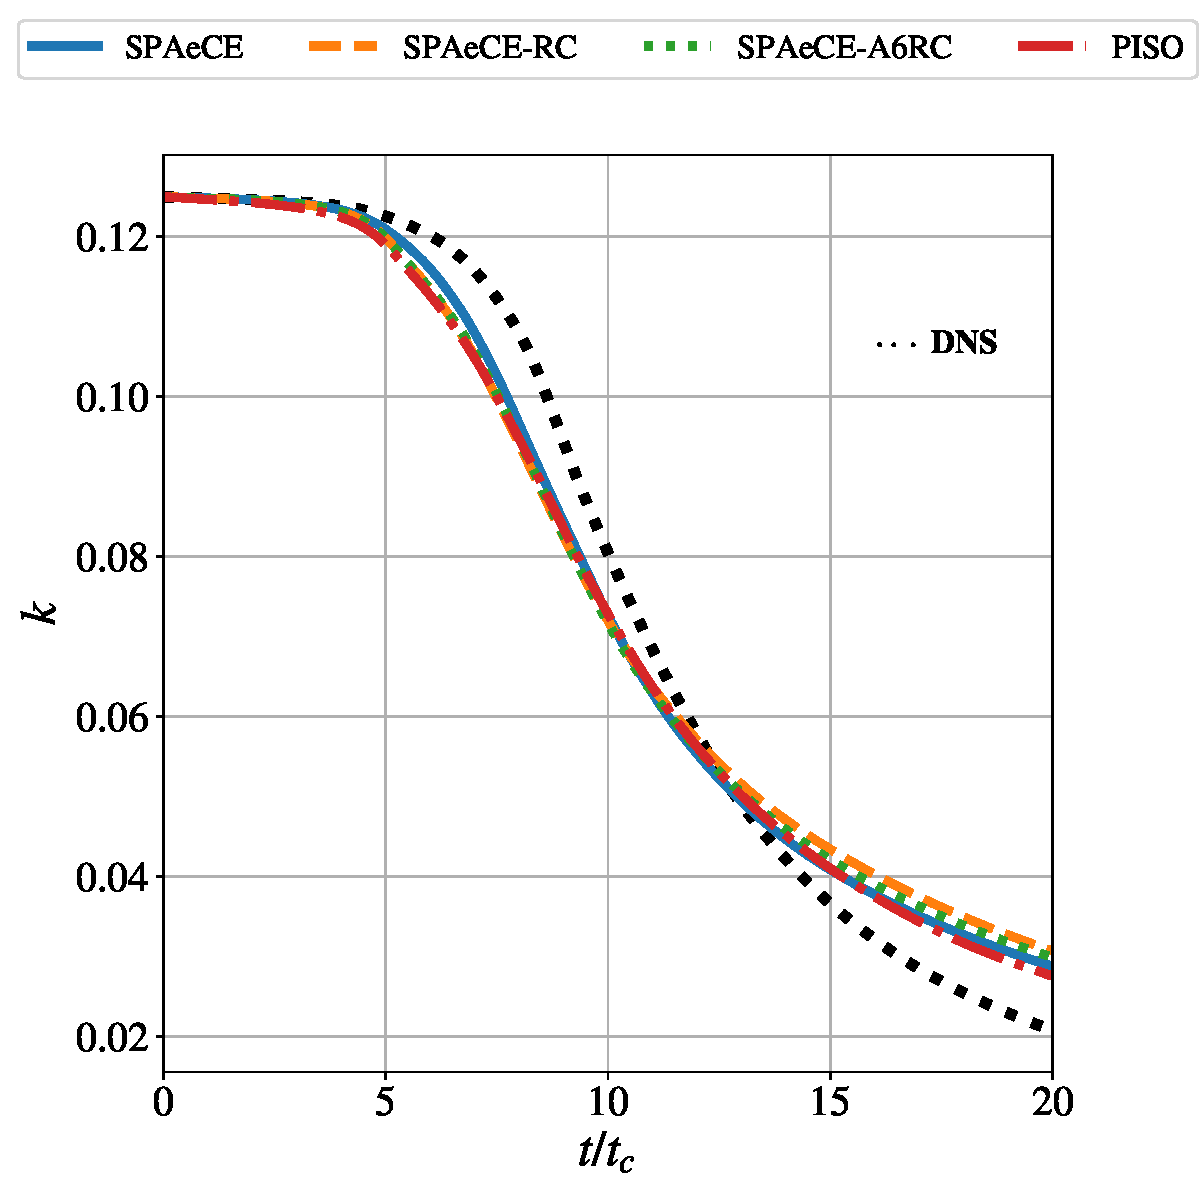
\includegraphics[width=\imgHalfWidth\columnwidth]{TGV3D/Re5000/spaeceFoamCNTGV/cubeVsPrism/65cubed/3DTGV_Re5000_spaeceFoamCNTGV_dynKEqnHeinz_8x8_k.pdf}\label{fig:TGV3Dcomp-k}}
\subfloat[KE decay rate \& dissipation rate]{\includegraphics[width=\imgHalfWidth\columnwidth]{TGV3D/Re5000/spaeceFoamCNTGV/cubeVsPrism/65cubed/3DTGV_Re5000_spaeceFoamCNTGV_dynKEqnHeinz_8x8_epsDkdt0.pdf}\label{fig:TGV3Dcomp-eps}} 
\caption{Comparison of \spaece algorithm KE decay (left), and KE decay rate and dissipation rate (right) in a 3D Taylor-Green vortex of $Re = 5\times10^3$ between a Cartesian cubic $65 \times 65 \times 65$ mesh and a right-angle prism $(65 \times 65) \times 2 \times 65$ mesh} 
\label{fig:TGV3Dcomp}
\end{figure}

In the right-angle prism mesh, the early oscillatory nature of the KE decay rate and dissipation rate (see Fig. \ref{fig:TGV3Dcomp-eps}) is due to the presence of strong checker-board like pattern, which results in increased dissipation and eventually, affected the KE evolution at all subsequent times. Overall, the \spaece algorithm produces no artificial dissipation in both orthogonal and non-orthogonal meshes, but the influence of mesh types remain.



%\clearpage
%\newpage
\subsection{Damping the high frequency modes}
\label{sec:dampHFModes}

In Sec. \ref{sec:advReg}, we have mentioned that $A6$ regularization when applied to the \spaece algorithm does not add any artificial dissipation. In Fig. \ref{fig:TGV3D-5k-A6} influence of $A6$ regularization in a 3D Taylor-Green vortex with $Re = 5 \time 10^3$ simulated in Cartesian cubic $65 \times 65 \times 65$ and $129 \times 129 \times 129$ mesh.

To model the sub-filter scales in the \spaece solver, the dynamic k equation turbulence model (cite Heinz) is used with the polyLaplace filter (Eq. \eqref{eqn:polyLaplace}) coefficient $\epsilon = 2$ and grid-spacing coefficient $\Delta =1$.  For the \spaeceA solver, the polyLaplace residual-filter (Eq. \eqref{eqn:resFilter}) with $\epsilon = 3,\,\Delta =1$ is used for regularization. Since the $A6$ method dampens the near-filter high frequency modes, the grid-spacing coefficient is raised to $\Delta =1.5$ and filter coefficient retained at $\epsilon = 2$ for SFS polyLaplace filter. There are slight difference in KE decay rate between the \spaece and \spaeceA algorithms, however in both meshes KE decay rate exactly matches with the total dissipation.

\begin{figure}[!h]
\centering
\subfloat[$65 \times 65 \times 65$ mesh]{\includegraphics[width=\imgHalfWidth\columnwidth]{TGV3D/Re5000/spaeceFoamCNTGV/spaeceVsSpaeceA6/65x65x65/3DTGV_Re5000_spaeceFoamCNTGV_dynKEqnHeinz_8x8_epsDkdt0.pdf}\label{fig:TGV3D-5k-A6-65}}
\subfloat[$129 \times 129 \times 129$ mesh]{\includegraphics[width=\imgHalfWidth\columnwidth]{TGV3D/Re5000/spaeceFoamCNTGV/spaeceVsSpaeceA6/129x129x129/3DTGV_Re5000_spaeceFoamCNTGV_dynKEqnHeinz_8x8_epsDkdt0.pdf}\label{fig:TGV3D-5k-A6-129}} 
\caption{$A6$ regularization does not add any dissipation} 
\label{fig:TGV3D-5k-A6}
\end{figure}

In addition to an artificial dissipation free regularization, the $A6$ advection regularization method redistributes energy from the near-filter-cutoff $\kappa_{cutoff}$, high frequency modes to the lower frequency modes by dissipating the high frequency modes faster than the inertial range cascade. 

To investigate influence of the $A6$ regularization, KE spectrum for the 3D Taylor-Green vortex at time $t/t_c =9$ is compared at Fig. \ref{fig:TGV3D-5k-A6Spec}. The \spaece algorithm demonstrated a constant slope at the inertial range. In case of the \spaeceA algorithm, the slope of the energy cascade gets steeper roughly from $k_{cutoff}/2$ to $k_{cutoff}$ wave-numbers. For the fine $129 \times 129 \times 129$ mesh, the \spaeceA algorithm successfully attenuated the high-frequency modes and obtained a better match with the KE spectrum.

\begin{figure}[!h]
\centering
\subfloat[$65 \times 65 \times 65$ mesh]{\includegraphics[width=\imgHalfWidth\columnwidth]{TGV3D/Re5000/spaeceVsSpaeceA6/65x65x65/spectrum/3DTGV5000-energySpectrum-dynKEqnHeinz-Time090.pdf}\label{fig:TGV3D-5k-A6Spec-65}}
\subfloat[$129 \times 129 \times 129$ mesh]{\includegraphics[width=\imgHalfWidth\columnwidth]{TGV3D/Re5000/spaeceVsSpaeceA6/129x129x129//spectrum/3DTGV5000-energySpectrum-dynKEqnHeinz-Time090.pdf}\label{fig:TGV3D-5k-A6Spec-129}} 
\caption{$A6$ dampens the high frequency modes} 
\label{fig:TGV3D-5k-A6Spec}
\end{figure}

Besides the 3D Taylor-Green vortex case, decay of an incompressible homogeneous isotropic turbulence case is also simulated following the experimental investigation performed by Comte-Bellot and Corrsin \cite{CBC1971}. Flow field measurements were performed at $Re = 3.4\times10^4$ with characteristic velocity (free-stream) $U_0 = 10\, m/s$ and characteristic length-scale (grid-spacing) $M = 5.08\, cm$ (or $2$ inch). Thus the molecular viscosity is $ \nu = \frac{U_0 M}{Re} = \frac{10 \times 0.0508}{3.4\times10^4} = 1.49412 \times10^{-4} \approx 1.5\times10^{-4} m^2/s$. In the reference experiment, turbulence kinetic energy (TKE) spectrum is computed at non-dimensional times of $t_c = \frac{U_0 t}{M} = 42,\, 98$ and $171$; equating to dimensional times of $0.213s,\, 0.498s$ and $0.869s$ respectively.

The computational domain comprises a 3D cube with side length of $9\times2\pi\, cm$. Initial turbulent velocity field at time $0.213s$ is generated using the OpenFOAM-v1912 \emph{createBoxTurb}\footnote{The createBoxTurb application implements the synthetic turbulence generation method proposed by Saad et al. \cite{Saad2016}; open source code available at: https://www.openfoam.com/documentation/guides/latest/man/createBoxTurb.html} utility following the corresponding turbulence kinetic energy spectrum reported by Comte-Bellot and Corrsin \cite[Table 3]{CBC1971}. The sub-filter stress in the \spaece and \spaeceA algorithms are modeled following the same approach as the 3D Taylor-Green vortex case. Finally, the Turbulence Kinetic Energy (TKE) spectrum is compared at times $t_c =98\, (t=0.498s)$ and $t_c =171\, (t=0.869s)$ (Fig. \ref{fig:HIT98}).

\begin{figure}[!h]
\centering
\subfloat[$65 \times 65 \times 65$]{\includegraphics[width=\imgHalfWidth\columnwidth]{HITCBC/65cubed/HIT-energySpectrum-Zoomed-Time98.pdf}\label{fig:HIT98-65}}
\subfloat[$129 \times 129 \times 129$]{\includegraphics[width=\imgHalfWidth\columnwidth]{HITCBC/129cubed/HIT-energySpectrum-Zoomed-Time98.pdf}\label{fig:HIT98-129}} 
\caption{Homogeneous isotropic turbulence } 
\label{fig:HIT98}
\end{figure}

%Introduce A6 correction: show results from HIT-CBC and 3D TGV Re 5000 cases.

In both test cases, the \spaeceA solver achieved significant improvement in KE spectrum match over the \spaece solver in the well resolved $129 \times 129 \times 129$ mesh (Fig. \ref{fig:HIT98-129}). However, for the coarse $65 \times 65 \times 65$ mesh, the $A6$ regularization seems to over dampen the near filter modes and energy accumulation is observed in the intermediate range(Fig. \ref{fig:HIT98-65}). Thus, use of $A6$ regularization to coarsely resolved mesh is not recommended!

Application of the $A6$ regularization in conjunction with Rhie-Chow correction deliver better results that application of Rhie-Chow correction alone! In the 3D Taylor-Green vortex of $Re = 5 \times 10^3$ simulation with Cartesian cubic mesh, \spaeceARC algorithm has less artificial dissipation (see Fig. \ref{fig:TGV3D-5k-A6RC}) and better spectrum match (see Fig. \ref{fig:TGV3dSpec}) compared to the \spaeceRC algorithm. The superiority of the \spaeceARC algorithm is more prominent in the coarse $65 \times 65 \times 65$ mesh than the fine $129 \times 129 \times 129$ mesh. The \piso algorithm displayed most non-physical dissipation and least spectrum match for both meshes. Therefore, \spaeceARC is our recommended algorithm, although the $A6$ regularization may increase the computational time to approximately $10 \%$ compared to the \spaeceRC algorithm.

% The $A6$ regularization redistributes energy from the high frequency modes to intermediate frequency modes, thus leaving less energy at high-frequecy modes which are most affection by the Rhie-Chow correction. In absence any regularization, the Rhie-Chow correction dissipates lot more energy, thus larger non-physical dissipation. % doulble check if its the implicit convection term and advection regularization?%

\begin{figure}[!h]
\centering
\subfloat[$65 \times 65 \times 65$ mesh]{\includegraphics[width=\imgHalfWidth\columnwidth]{TGV3D/Re5000/pisoVsSpaeceRCVsSpaeceA6RC/65x65x65/3DTGV_Re5000_dynKEqnHeinz_8x8_nuEff.pdf}\label{fig:TGV3D-5k-A6RC-65}}
\subfloat[$129 \times 129 \times 129$ mesh]{\includegraphics[width=\imgHalfWidth\columnwidth]{TGV3D/Re5000//pisoVsSpaeceRCVsSpaeceA6RC/129x129x129/3DTGV_Re5000_dynKEqnHeinz_8x8_nuEff.pdf}\label{fig:TGV3D-5k-A6EC-129}} 
\caption{$A6RC$ regularization better than RC} 
\label{fig:TGV3D-5k-A6RC}
\end{figure}


\begin{figure}[!h]
\centering
\subfloat[$65 \times 65 \times 65$]{\includegraphics[width=\imgHalfWidth\columnwidth]{TGV3D/Re5000/pisoVsSpaeceRCVsSpaeceA6RC/65x65x65/spectrum/3DTGV5000-energySpectrum-dynKEqnHeinz-Time090.pdf}\label{fig:TGV3dSpec-65}}
\subfloat[$129 \times 129 \times 129$ mesh]{\includegraphics[width=\imgHalfWidth\columnwidth]{TGV3D/Re5000/pisoVsSpaeceRCVsSpaeceA6RC/129x129x129/spectrum/3DTGV5000-energySpectrum-dynKEqnHeinz-Time090.pdf}\label{fig:TGV3dSpec-129}} 
\caption{\spaeceARC match KE spectrum better than the \piso} 
\label{fig:TGV3dSpec}
\end{figure}


\clearpage
\newpage

